<<<<<<< current
%!TEX root = ../thesis.tex
%*******************************************************************************
%****************************** Third Chapter **********************************
%*******************************************************************************
\chapter{Pose estimation using a single camera}%Lateral and height

% **************************** Define Graphics   Path **************************
\ifpdf
    \graphicspath{{Chapter3/Figs/Raster/}{Chapter3/Figs/PDF/}{Chapter3/Figs/}}
\else
    \graphicspath{{Chapter3/Figs/Vector/}{Chapter3/Figs/}}
\fi


UAV autonomous navigation into corridors or tunnels is a hard task due mainly to the localization problem. GPS measurements are usually dropped noised or unavailable. Cameras become a popular sensors for pose estimation even if sometimes is hard to compute on-board the algorithm. This chapter is centered on the estimation of the relative position of the vehicle through a single image in real-time execution. This information is useful since it serves to make an indoor navigation (in a corridor). The algorithm designed is intended to use the minimum of resources of the computer. Although this first stage focuses on using tools such as matlab, the algorithms can be easily implemented in an embedded system. So the program can be resume as follow: firstly the virtual image is obtained. Then the edges of the image are extracted.  The rotation %This extracted information are all the lines obtained from the edges of doors, windows, walls, corners, etc.
matrix of the camera is estimated using infinite vanishing points and finite vanishing points. A new sub-classification of lines is made from the finite vanishing point. This subset is done in four quadrants. Using the finite vanishing point and the information of each quadrant, we can obtain the principal line from each corner. The collinearity property is used with pairs of major lines. If there is a collinearity between each pair of lines the system is centered. Otherwise, the result is a percentage of displacement in the \textit{y}-axis, \textit{z}-axis.  The scale is a percentage of displacement where the center of the corridor indicates a zero percentage of displacement. A numerical validation is made in order to verify this algorithm.

\section{Pose estimation algorithm}

 The proposed vision algorithm takes into account the perspective projection, the vanish point identification and the collinearities of the principal lines in the image to estimate the pose of an aerial vehicle. 0.2cm Ideas from \cite{Akinlar2011, boulanger:inria-00461526} and \cite{Lee2009} have inspired our algorithm.  The general scheme of the estimation pose algorithm can be seen in Figure \ref{fig:1_algo}. As can be observed in this figure, once the image is acquired a line
detector algorithm is applied. For making a subset of vertical, horizontal and diagonal lines a histogram is then used. After that, the rotation matrix is acquired and the line classification algorithm is again applied for extracting principal lines in the image. This information is used with the collinearity approach for estimating the pose of the camera. Therefore it is relatively easy compute the \textit{y} and \textit{z}-axis in the image plane.

Figure \ref{fig:VisionAlgoritm} shows the general procedure, and  this  depics too the vanishing point evolution. For obtaining the pose estimation it is necessary to know the camera model, next subsections will introduce this concept and each block in the general scheme algorithm.

\begin{figure*}[h!]
\centering
\includegraphics[width=0.85\textwidth]{Chapter03/Images/Algoritme_m.png}
\caption{These images introduce the applied methodology. The scene is a corridor and an image is taken from the video to extract a set of lines that could describe geometrically the environment and the rotation matrix. Four new subsets of lines are made taking into account the vanishing point (quadrant 1, 2, 3 and 4). The information of each quadrant is used to obtain the principal lines (LQ1, LQ2, LQ3, LQ4). }
\label{fig:VisionAlgoritm}
\end{figure*}


\subsection{Vanishing point algorithm}
Perspective projection of parallel lines in world space creates vanishing lines in image space that
intersect in a point called vanishing point. If the parallel lines are parallel to the image plane,
the vanishing lines are also parallel to this plane and the vanishing point is at an infinite
distance from the image center, hence is called infinite vanishing point. Otherwise, it is a finite
vanishing point. For our case the camera calibration is based on the following assumption: the main vanishing lines in the input image correspond to three orthogonal directions in world space as can be seen in Figure \ref{fig:VisionAlgoritm}.

\subsection{Dominant lines detection}
In man-made indoor environments, it is possible to extract line segments, texture, colors and so on.
In this work,  the linear time line segment detector called EDlines \cite{Akinlar2011} is used giving accurate results and with high time process (all the segments for an image $240 \times3 20$ are computed in 3 $ms$). This algorithm no requires parameter tuning and run ups faster than others methods as the Hough transform \cite{HoughMAtlab}.

\subsection{Lines classification}

RANSAC (Random Sample Consensus) has become  a simple and powerful method to %various authors have been developed and introduced RANSAC as
provide a partition of parallel straight lines into clusters by
pruning outliers. \color{blue} The algorithm begins selecting randomly  two lines for generating a VP hypothesis.  These lines  are grouped together in order to optimize the estimated VP and for obtaining a dominant VP.
When a dominant VP is obtained, the process finishes. Nevertheless, several finite vanishing points can be
extracted from the environment with this algorithm. \color{black} \vskip 0.2cm


In the context of indoor navigation, the main orthogonal
directions in environments consist generally in a vertical
one (often associated with an infinite VP) and two horizontal
ones (associated with finite or infinite VP). In this work, the heuristic strategy is taken  to extract a
limited number of reliable VP while enforcing the
orthogonality constraint, in conjunction with RANSAC.  \vskip 0.2cm

For a robust selection of VPs, an histogram is made in order to classify
all the set of lines in a subset of vertical lines  $L_v$, a subset of horizontal lines $L_h$ and a subset
of diagonal lines $L_d$. For clustering lines by RANSAC, the consensus score is quite different
depending on each subset and is computing with (\ref{RansacVP1}). Unlike the finite VP whose coordinates may be determined in
the image plan (lines $L_d$), the infinite VPs are generally represented with a
direction (lines $L_v$, $L_h$). For finite VP, the consensus score is based on a
distance between the candidate straight line and the
intersecting point and represented as (\ref{RansacVP2}). For infinite VP, it is obtained with (\ref{RansacIVP}) using the angular
distance between the direction of the candidate straight line
and the direction representing the infinite VP,  more details see \cite{Elloumi2014}.

\begin{eqnarray}
	score &=&  \sum_{i=0}^{n} \Upsilon(v,l_i)  \label{RansacVP1} \\
  	\Upsilon(v,l_i)  &=&  \left \{\begin{array}{ll}
 	                   1 & d(v,l_i) < \delta\\
 	                   0 &  \text{otherwise}
 	                  \end{array} \right.       \label{RansacVP2} \\
	 \Upsilon(v,l_i) &=&  \left \{\begin{array}{ll}
 	                   1 & Min(\widehat{(\overrightarrow{v},\overrightarrow{l_i})},\widehat{(\overrightarrow{l_i},\overrightarrow{v})}) < \delta\\
 	                   0 & \text{otherwise}
 	                  \end{array} \right.   \label{RansacIVP}
 \end{eqnarray}
where $n$ is the number of dominant lines and $d(v, l_i)$ denotes the
Euclidian distance from the finite VP candidate $v$ to the line $l_i$.
The lines whose distance is below a fixed threshold $\delta$ are
considered as participants. $(\overrightarrow{v},\overrightarrow{l_i})$ describes the angle between the infinite VP direction
from the image center and the line $l_i$ to test in image space. \color{black}

\subsection{Rotation matrix estimation}

It is known that when using the VPs intrinsic and extrinsic camera parameters can be estimated. We consider that the intrinsic parameters are known thus we will focus on compute the others ones, in particularly the Rotation matrix.
The main point $p$ of the camera is set to the center of the image plane. The rotation matrix
$(\vec{u},\vec{v},\vec{w})$ transforms points from real world to the image plane. Its columns are the vectors of the world coordinates frame expressed in the camera space. The directions of the three vanishing points from the optical center of the camera are assumed to be orthogonal. Thus without loss of generality, the following relations hold for the final calibrated.

% \begin{subequations}
% \begin{align}
% 	\label{VectorOrto}
% 	f>0 \\
% 	\vec{u} \cdot \vec{v}= \vec{v}\cdot \vec{w}=\vec{w}\cdot \vec{u}=0\\
%   	\abs{\vec{u}}=\abs{\vec{v}}=\abs{\vec{w}}
% \end{align}
% \end{subequations}

The obtained structured lines  from the corridor image provide enough information to estimate the camera rotation matrix.
Normally, it is supposed that the camera has a vertical position, and  as the corridor is plenty of vertical and horizontal lines, then it is possible to find a finite vanishing point and two infinite vanishing points.


\subsubsection*{A finite vanishing point, two infinite vanishing points}

\begin{figure}[h!]
\centering
\includegraphics[width=0.8\textwidth]{Chapter03/Images/twoInfiniteVPOneFVPG.pdf}
\caption{Camera calibration with one finite and two infinite vanishing points. $(x_c,y_c,z_c)$ is the camera coordinate frame, $(\vec{u},\vec{v},\vec{w})$ the world coordinate frame, $VP$ the finite vanishing point, $\vec{I_1}$ and $\vec{I_2}$ the infinite vanishing point directions. $P$ is the main point.}
\label{fig:3_unpunto}
\end{figure}

This case occurs when two axes of the world frame are parallel to the image plane.  Fig \ref{fig:3_unpunto}
introduces the terms involved for the camera calibration
using one finite vanishing point $\overrightarrow{OVP} = (vp_{x}, vp_{y},-f )^T$ and
two infinite vanishing points with directions $\vec{I_1} = (I_{1_x}, I_{1_y},0)^T$
and $\vec{I_2} = (I_{2_x}, I_{2_y},0)^T$. \vskip 0.2cm


The vector $\vec{w}'$ defines a non-normalized form of  $\vec{w}$,
and is computed from the finite vanishing point as
\begin{equation}
	\label{oneVanish}
	\vec{w}'= (w_{x}',w_{y}',w_{z}')=\overrightarrow{OVP}=(vp_{x}, vp_{y},-f )
 \end{equation}

The coordinate axis $\vec{u}$, as indicated in Figure \ref{fig:3_unpuntoH}, lies
on the plane defined by the points $O$, $P$ and the direction
$\vec{I_1} = (I_{1_x}, I_{1_y},0)^T$ . Then $\vec{u}'$, the non-normalized version of
$\vec{u}$, can be expressed as $\vec{u}' = (I_{1_x}, I_{1_y},u_{z}')$. The goal is that
$\vec{u}$ and $\vec{w}$ belong into an orthogonal coordinate frame, then
\begin{equation}
	%\label{oneVanish}
	\vec{u}' \cdot  \vec{w}'= I_{1_x}w_{x}'+ I_{1_y}w_{y}'+u_{z}'w_{z}' =0
 \end{equation}
therefore
 \begin{equation}
	\label{PlanoU}
	u_{z}'=\frac{I_{1_x}w_{x}'+ I_{1_y}w_{y}'}{f}
\end{equation}

\begin{figure}[h]
\centering
\includegraphics[scale=0.5]{Chapter03/Images/twoInfiniteVPOneFVPH.pdf}
\caption{ $\vec{u}$ estimation from the infinite vanishing points.}
\label{fig:3_unpuntoH}
\end{figure}

Similar procedures can be used for $\vec{v}' = (I_{2_x}, I_{2_y},v_{z}')$ (see Figure \ref{fig:3_unpuntoV}), thus

\begin{equation}
	\label{PlanoV}
	v_{z}'=\frac{I_{2_x}w_{x}'+ I_{2_y}w_{y}'}{f}
\end{equation}

\begin{figure}[h]
\centering
\includegraphics[scale=0.5]{Chapter03/Images/twoInfiniteVPOneFVPV.pdf}
\caption{$\vec{v}$ estimation from  the infinite vanishing points.}
\label{fig:3_unpuntoV}
\end{figure}

Typically the vertical lines are plenty and more precise in
many images, so it retains $\vec{v}'$ and $\vec{w}'$ and compute $\vec{u}'$ using a
cross product, $\vec{u}'= \vec{v}'\times \vec{w}'$. The rotation matrix of the camera $R= (\vec{u},\vec{v},\vec{w})$ from
 Eq. (\ref{CameraMatrix}) which meets the conditions from Eq. (\ref{VectorOrto}) is
obtained by normalizing $\vec{u}'$, $\vec{v}'$ and $\vec{w}'$.


\subsection{Principal lines estimation}

color{blue}

Once the camera rotation matrix obtained, fusing this information with $ L_v $,  $ L_h $ and  $ L_d $ thus, the principal lines of the corridor (corners of the the corridor) could be estimated. The algorithm results in  four new subsets (quadrants 1,2,3,4) relatives with to the vanishing point and the rotation matrix. Therefore, the information in each quadrant
is useful to find the main line of each subset. Each subset of lines contains the beginning and end point of each line as well as its inclination and its length.  \vskip 0.2cm

\color{magenta}

The principal lines which are in the border of the right wall-ceiling $L_{Q_1}$, right wall-floor $L_{Q_2}$,
left wall-ceiling $L_{Q_3}$ and left wall-floor $L_{Q_4}$ are depicted in Fig \ref{fig:VisionAlgoritm}.  \vskip 0.2cm

% \subsubsection{Generalized least squares fitting}

%{\footnotesize
%      \begin{tabular}{p{0.6\textwidth} p{0.4\textwidth}}
	%  \begin{itemize}
%     \item Let  $X_1=(x_1,x_2,...,x_n)^T$ and $Y_1=(y_1,y_2,...,y_n)^T$. Define a new $2\times n$ matrix $X=(X_1, Y_1)^T$.
%    {\tiny

   \begin{equation*}
 C_m\equiv \begin{bmatrix}%\dfrac{1}{2}XX^T=
     \omega_n \sum x_n^2   &  \omega_n \sum x_n y_n \\
     \omega_n \sum x_n y_n &  \omega_n \sum y_n^2
    \end{bmatrix}
\end{equation*}
%}

$(x_n,y_n)$ are the initial and final points from each line, $C_m$ represents the covariance matrix, $m$ represents the frames and
\begin{equation*}
 \omega_n=e^{\frac{-0.5 \theta^2}{\sigma^2}}
\end{equation*}
\begin{equation*}
 \theta=\arctan \frac{x_n a_{m-1}+y_n b_{m-1}}{x_n a_{m-1}-y_n b_{m-1}}
\end{equation*}

Where $\omega_n$ is the weight that supply the response variance to a constant value, $a_{m-1}, b_{m-1}$ represents initial line hypothesis and the .


\begin{equation*}
y=LQ_k=-\frac{b_m}{a_m} x
\end{equation*}
where the vector proper  $\alpha=[a_m, b_m]^T$ extracted from $C_m$ represents the principal line of each quadrant with $k=1,2,3,4$.

\color{red}
Sigo sin entender esta ultima parte que me enviaste
podrias explicarlo en espanol?
\color{black}

\subsection{Pose camera estimation}


\color{blue}

Position camera estimation is obtained using the previous results and the relation with the borders of the corridor. Hence, when the camera is in the center of the corridor, there is a collinearity
between the lines $L_{Q_1},L_{Q_3}$ and $L_{Q_2},L_{Q_4}$ that can be expressed as
\begin{eqnarray}
		   CP_{1,3} &=& L_{Q_1}\wedge L_{Q_3} \label{crossLines13} \\
		   CP_{2,4} &= & L_{Q_2}\wedge L_{Q_4} \label{crossLines24}
\end{eqnarray}

The third component of $CP_{1,3}$ and $CP_{2,4}$ supplies the information to obtain the relative camera position and it is given as
\begin{eqnarray}
		y_r=CP_{1,3}-CP_{2,4} \label{relaitve_x} \\
z_r=CP_{1,3}+CP_{2,4} \label{realitive_z}
\end{eqnarray}
where $y_r$ and $z_r$ are the relative position with respect to the center of the corridor. \\

\color{black}

\color{red}
Las figuras que pusiste y como las pusiste no se ven, tienden a confundir y hace mas complicado el asunto para entender, te voy a poner un bosquejo de como quedaria mejor..
para esto necesito una secuencia de estas figuras separadas (cada figura separada..)
\color{blue}

\section{Numerical validation}
%

The previous algorithm for pose estimation was firstly tested off-line. For corroborating equations (\ref{crossLines13}) and (\ref{crossLines24}) a sequence of images where taken with specified  movements as shown in Figures \ref{camera up and down} and \ref{camera right and left}.

\begin{figure} [h!]
\centering
\includegraphics[scale=0.5]{Chapter03/Images/CentreFrames_m.png}
\caption{Pictures with a camera in the middle of a corridor. The test was: 1) stay at the middle, 2) move up, 3) returns to the middle, 4) move down and 5) returns to the middle. }
\label{camera up and down}
\end{figure}


\begin{figure} [h!]
\centering
\includegraphics[scale=0.5]{Chapter03/Images/Lateral_m.png}
\caption{Pictures with a camera in the middle of a corridor. The test was: 1) stay at the middle, 2) move rigth, 3) returns to the middle, 4) move left and 5) returns to the middle. }
\label{camera right and left}
\end{figure}

The experiment was to place the camera in the middle of the corridor and moves it firstly up and down (Figure \ref{camera up and down}) and after right and left (Figure \ref{camera right and left}). These movements can be represented via principal lines in the image and observed graphically in Figures  \ref{fig:CentreFrames} and \ref{fig:lateralFRames}, where the cross product between $L_{Q_i}$ are represented, see (\ref{crossLines13}) and (\ref{crossLines24}). On one hand, notice for example from Figure \ref{fig:CentreFrames}  that both cross products have the same behavior and when if the camera is moved up the lines representing $L_{Q_1}\wedge L_{Q_3}$  and $L_{Q_4}\wedge L_{Q_2}$ increase and when the camera is moved down they decrease, representing then the good camera's behavior. On the other hand, when the camera is moved right and left, then the cross product between $L_{Q_1}\wedge L_{Q_3}$  and $L_{Q_4}\wedge L_{Q_2}$ are different (see Figure  \ref{fig:lateralFRames}), nevertheless this information gives necessary data to estimate the $y$ position, as can be seen in Figure  \ref{fig:XYlateral}. Observe in this figure that when the camera is moved right the $y$ estimation is negative and if it is moved left, then a $y$ positive response is obtained. In addition note that $z$ estimation remains quasi-constant. Similarly for Figure \ref{fig:XYcentre} where with the up and down camera's movements the $z$ state is estimated, observe also that $y$ estimation is also quasi-constant.



\begin{figure}[h!]
        \centering
        % This file was created by matlab2tikz.
% Minimal pgfplots version: 1.3
%
%The latest updates can be retrieved from
%  http://www.mathworks.com/matlabcentral/fileexchange/22022-matlab2tikz
%where you can also make suggestions and rate matlab2tikz.
%
\definecolor{mycolor1}{rgb}{0.00000,0.44700,0.74100}%
\definecolor{mycolor2}{rgb}{0.85000,0.32500,0.09800}%
%
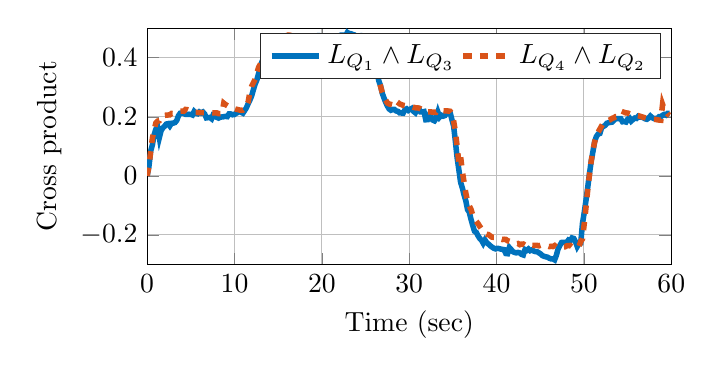
\begin{tikzpicture}

\begin{axis}[%
width=6.656442cm,
height=3cm,
at={(0cm,0cm)},
scale only axis,
xmin=0,
xmax=60,
xlabel={Time (sec)},
xmajorgrids,
ymin=-0.3,
ymax=0.5,
ylabel={Cross product},
ymajorgrids,
legend style={legend columns=2,legend cell align=left,align=left,draw=white!15!black}
]
\addplot [color=mycolor1,solid,line width=2.0pt]
  table[row sep=crcr]{%
0	0\\
0.199335548172757	0.030742027925972\\
0.398671096345515	0.0828735307141348\\
0.598006644518272	0.105081321825358\\
0.79734219269103	0.138826415767478\\
0.996677740863787	0.158012182380284\\
1.19601328903654	0.165318336971575\\
1.3953488372093	0.129759187651805\\
1.59468438538206	0.153461059573169\\
1.79401993355482	0.162469237192847\\
1.99335548172757	0.167889162514036\\
2.19269102990033	0.175363911624859\\
2.39202657807309	0.17679802060079\\
2.59136212624585	0.169046976759301\\
2.7906976744186	0.17803807773658\\
2.99003322259136	0.17865142111461\\
3.18936877076412	0.180553164243146\\
3.38870431893688	0.187710505101491\\
3.58803986710963	0.204041035478399\\
3.78737541528239	0.21217945191349\\
3.98671096345515	0.21305849534408\\
4.18604651162791	0.211274427028537\\
4.38538205980066	0.208293620013859\\
4.58471760797342	0.20836783661539\\
4.78405315614618	0.208628644841035\\
4.98338870431894	0.208369223901828\\
5.18272425249169	0.206154168791621\\
5.38205980066445	0.21778747263864\\
5.58139534883721	0.211650949117691\\
5.78073089700997	0.210224040265121\\
5.98006644518272	0.216316680182076\\
6.17940199335548	0.212784544860855\\
6.37873754152824	0.216163792212759\\
6.578073089701	0.210087929923006\\
6.77740863787375	0.196315112872329\\
6.97674418604651	0.197105507459289\\
7.17607973421927	0.197806072188377\\
7.37541528239203	0.193373638163163\\
7.57475083056478	0.208069099458681\\
7.77408637873754	0.208034793813171\\
7.9734219269103	0.198240381391177\\
8.17275747508306	0.195685221835226\\
8.37209302325581	0.198911960913538\\
8.57142857142857	0.19944310829398\\
8.77076411960133	0.200307530669613\\
8.97009966777409	0.201433223855905\\
9.16943521594684	0.200608875718738\\
9.3687707641196	0.209704024239964\\
9.56810631229236	0.209636210457107\\
9.76744186046512	0.206945066931917\\
9.96677740863787	0.20756166503172\\
10.1661129568106	0.211824702244533\\
10.3654485049834	0.214729736631606\\
10.5647840531561	0.218446630875855\\
10.7641196013289	0.215449324758097\\
10.9634551495017	0.212325909892533\\
11.1627906976744	0.221127132960991\\
11.3621262458472	0.230712638671687\\
11.5614617940199	0.244434338600201\\
11.7607973421927	0.256643111495394\\
11.9601328903654	0.270713831033366\\
12.1594684385382	0.291476166526801\\
12.358803986711	0.310759262817296\\
12.5581395348837	0.32485284027707\\
12.7574750830565	0.346592051833787\\
12.9568106312292	0.369733610076934\\
13.156146179402	0.387575727549183\\
13.3554817275748	0.400630217873027\\
13.5548172757475	0.406061953187462\\
13.7541528239203	0.4202093386277\\
13.953488372093	0.426108587752899\\
14.1528239202658	0.433045756421874\\
14.3521594684385	0.440076903749821\\
14.5514950166113	0.444816326368204\\
14.7508305647841	0.450248529944735\\
14.9501661129568	0.452032845365701\\
15.1495016611296	0.456702468586884\\
15.3488372093023	0.457721551086022\\
15.5481727574751	0.456476945481678\\
15.7475083056478	0.456228382158606\\
15.9468438538206	0.457351532254795\\
16.1461794019934	0.458873391847378\\
16.3455149501661	0.460155924541988\\
16.5448504983389	0.463836678313106\\
16.7441860465116	0.46708914589731\\
16.9435215946844	0.467229370585945\\
17.1428571428571	0.468814394298497\\
17.3421926910299	0.467151525259722\\
17.5415282392027	0.469992125696965\\
17.7408637873754	0.470488153561163\\
17.9401993355482	0.47133828366119\\
18.1395348837209	0.4712136054494\\
18.3388704318937	0.473197952459583\\
18.5382059800664	0.473811810239429\\
18.7375415282392	0.473721931121786\\
18.936877076412	0.474306122558772\\
19.1362126245847	0.473769240182764\\
19.3355481727575	0.471807952378505\\
19.5348837209302	0.475075360110677\\
19.734219269103	0.474889855501165\\
19.9335548172757	0.471753722095564\\
20.1328903654485	0.471711717964217\\
20.3322259136213	0.471434487222184\\
20.531561461794	0.471181142315513\\
20.7308970099668	0.471324136765159\\
20.9302325581395	0.47165937825952\\
21.1295681063123	0.471579238738933\\
21.3289036544851	0.471649215234227\\
21.5282392026578	0.471422751723768\\
21.7275747508306	0.471064366542006\\
21.9269102990033	0.471177084730362\\
22.1262458471761	0.476173602152583\\
22.3255813953488	0.476317277665897\\
22.5249169435216	0.476468981081323\\
22.7242524916944	0.474890491991672\\
22.9235880398671	0.485672390921398\\
23.1229235880399	0.481640805503392\\
23.3222591362126	0.481305711319191\\
23.5215946843854	0.479101891431731\\
23.7209302325581	0.477222689645709\\
23.9202657807309	0.46995585831105\\
24.1196013289037	0.470143173565368\\
24.3189368770764	0.471353888074935\\
24.5182724252492	0.474670849246479\\
24.7176079734219	0.474214982532677\\
24.9169435215947	0.473309232825266\\
25.1162790697674	0.4702148595381\\
25.3156146179402	0.466623685141034\\
25.514950166113	0.458434098808722\\
25.7142857142857	0.431922133556878\\
25.9136212624585	0.406036866021997\\
26.1129568106312	0.38039995269299\\
26.312292358804	0.356831546083206\\
26.5116279069767	0.322200657313163\\
26.7109634551495	0.305814299966114\\
26.9102990033223	0.280394856478819\\
27.109634551495	0.263781848291225\\
27.3089700996678	0.248955514608588\\
27.5083056478405	0.236306847625229\\
27.7076411960133	0.226281537481772\\
27.906976744186	0.222261370563225\\
28.1063122923588	0.224721022706015\\
28.3056478405316	0.22476533346158\\
28.5049833887043	0.219702791930158\\
28.7043189368771	0.218639125249466\\
28.9036544850498	0.213235288983912\\
29.1029900332226	0.212913375488299\\
29.3023255813953	0.21228176757624\\
29.5016611295681	0.223800534132015\\
29.7009966777409	0.226901606259314\\
29.9003322259136	0.221722406316364\\
30.0996677740864	0.225702789436084\\
30.2990033222591	0.228714968858014\\
30.4983388704319	0.218398774482463\\
30.6976744186047	0.213802060701838\\
30.8970099667774	0.225847310857305\\
31.0963455149502	0.227346203360617\\
31.2956810631229	0.216690547489862\\
31.4950166112957	0.216552662799759\\
31.6943521594684	0.217670360719735\\
31.8936877076412	0.189999617580706\\
32.093023255814	0.19020693329187\\
32.2923588039867	0.20531608916418\\
32.4916943521595	0.201752114776826\\
32.6910299003322	0.189051967535848\\
32.890365448505	0.186402236710532\\
33.0897009966777	0.195223273001069\\
33.2890365448505	0.21553877298573\\
33.4883720930233	0.199105585068201\\
33.687707641196	0.205330469090425\\
33.8870431893688	0.20231250412812\\
34.0863787375415	0.204315298733265\\
34.2857142857143	0.213043572400633\\
34.485049833887	0.216381165891312\\
34.6843853820598	0.214338312518101\\
34.8837209302326	0.190891845755397\\
35.0830564784053	0.169045388129524\\
35.2823920265781	0.117970056131066\\
35.4817275747508	0.0618122169285922\\
35.6810631229236	0.0212892341015012\\
35.8803986710963	-0.021581250796285\\
36.0797342192691	-0.0407628403912041\\
36.2790697674419	-0.0643765588041649\\
36.4784053156146	-0.0845714012217986\\
36.6777408637874	-0.114381902194977\\
36.8770764119601	-0.123194462033602\\
37.0764119601329	-0.14726030403955\\
37.2757475083056	-0.16825262185245\\
37.4750830564784	-0.187557341614786\\
37.6744186046512	-0.19123943099753\\
37.8737541528239	-0.20267788063962\\
38.0730897009967	-0.211819315074755\\
38.2724252491694	-0.217778009185701\\
38.4717607973422	-0.228140241975077\\
38.671096345515	-0.217250594700689\\
38.8704318936877	-0.226107038531323\\
39.0697674418605	-0.23101328496671\\
39.2691029900332	-0.236516404359276\\
39.468438538206	-0.241075317536677\\
39.6677740863787	-0.244948723856249\\
39.8671096345515	-0.247255132191605\\
40.0664451827243	-0.245453814770265\\
40.265780730897	-0.246176164527333\\
40.4651162790698	-0.247822375278133\\
40.6644518272425	-0.249055730427652\\
40.8637873754153	-0.250090430167425\\
41.063122923588	-0.263017147931831\\
41.2624584717608	-0.263663827137829\\
41.4617940199336	-0.242798079796263\\
41.6611295681063	-0.24919543837436\\
41.8604651162791	-0.256558503461077\\
42.0598006644518	-0.259350205694448\\
42.2591362126246	-0.260856593203861\\
42.4584717607973	-0.259369184086433\\
42.6578073089701	-0.260847042991638\\
42.8571428571429	-0.265856079830801\\
43.0564784053156	-0.267909493358909\\
43.2558139534884	-0.249627090506112\\
43.4551495016611	-0.252631241082031\\
43.6544850498339	-0.24767615356644\\
43.8538205980066	-0.253337795568863\\
44.0531561461794	-0.250813819942353\\
44.2524916943522	-0.254503959520435\\
44.4518272425249	-0.256560896988312\\
44.6511627906977	-0.256939124807369\\
44.8504983388704	-0.260644196262074\\
45.0498338870432	-0.26467599272932\\
45.2491694352159	-0.270060067743338\\
45.4485049833887	-0.272537541860207\\
45.6478405315615	-0.274229327053171\\
45.8471760797342	-0.275545675048239\\
46.046511627907	-0.279129379972995\\
46.2458471760797	-0.281198619991069\\
46.4451827242525	-0.28133388193592\\
46.6445182724253	-0.284666226184072\\
46.843853820598	-0.269029365875755\\
47.0431893687708	-0.247307299970423\\
47.2425249169435	-0.235748069151903\\
47.4418604651163	-0.225715507665264\\
47.641196013289	-0.225238129680491\\
47.8405315614618	-0.225433256373713\\
48.0398671096346	-0.225339898102067\\
48.2392026578073	-0.217279286472469\\
48.4385382059801	-0.21950817849527\\
48.6378737541528	-0.21034184070411\\
48.8372093023256	-0.212044448467703\\
49.0365448504983	-0.222970250691113\\
49.2358803986711	-0.239279839462634\\
49.4352159468439	-0.229448609262718\\
49.6345514950166	-0.227709614278369\\
49.8338870431894	-0.161321648091734\\
50.0332225913621	-0.125025189719276\\
50.2325581395349	-0.0836592328544258\\
50.4318936877076	-0.0398627348046633\\
50.6312292358804	0.00644523607091106\\
50.8305647840532	0.0489271269236699\\
51.0299003322259	0.0817933479629508\\
51.2292358803987	0.116461406303344\\
51.4285714285714	0.133142431877358\\
51.6279069767442	0.141687609276178\\
51.8272425249169	0.143640859102146\\
52.0265780730897	0.163266584448222\\
52.2259136212625	0.167208817911571\\
52.4252491694352	0.170736927140942\\
52.624584717608	0.178133943399358\\
52.8239202657807	0.180061169482605\\
53.0232558139535	0.180927859896376\\
53.2225913621263	0.181934431053367\\
53.421926910299	0.188007236741809\\
53.6212624584718	0.193329091764933\\
53.8205980066445	0.193715212411015\\
54.0199335548173	0.193450778499299\\
54.21926910299	0.193539146654546\\
54.4186046511628	0.183228797260322\\
54.6179401993356	0.18367127988381\\
54.8172757475083	0.182204850007427\\
55.0166112956811	0.192454709402846\\
55.2159468438538	0.195686603320542\\
55.4152823920266	0.185684729861345\\
55.6146179401993	0.190869703698701\\
55.8139534883721	0.195644283409796\\
56.0132890365449	0.194616307400244\\
56.2126245847176	0.201526368934063\\
56.4119601328904	0.199051661999297\\
56.6112956810631	0.198620778169795\\
56.8106312292359	0.196725532921711\\
57.0099667774086	0.193020051971268\\
57.2093023255814	0.191649981814679\\
57.4086378737542	0.195882780971597\\
57.6079734219269	0.202607878832124\\
57.8073089700997	0.197014402839495\\
58.0066445182724	0.19407472768477\\
58.2059800664452	0.194624427427319\\
58.4053156146179	0.194431061787678\\
58.6046511627907	0.200303432988159\\
58.8039867109635	0.200403545770639\\
59.0033222591362	0.20509426583411\\
59.202657807309	0.208041508591756\\
59.4019933554817	0.205603969967094\\
59.6013289036545	0.211738682009683\\
59.8006644518272	0.211399667764344\\
};
\addlegendentry{$\text{L}_{\text{Q}_\text{1}}\wedge\text{L}_{\text{Q}_\text{3}}$};

\addplot [color=mycolor2,dashed,line width=2.0pt]
  table[row sep=crcr]{%
0	0\\
0.199335548172757	0.0320626091915426\\
0.398671096345515	0.0817511843045116\\
0.598006644518272	0.127257203409701\\
0.79734219269103	0.154878094363065\\
0.996677740863787	0.179061563427889\\
1.19601328903654	0.185412066139698\\
1.3953488372093	0.186713908020985\\
1.59468438538206	0.200172253811674\\
1.79401993355482	0.201408954219292\\
1.99335548172757	0.20493449428673\\
2.19269102990033	0.205666676396152\\
2.39202657807309	0.206091359201615\\
2.59136212624585	0.206554749313233\\
2.7906976744186	0.211245329020206\\
2.99003322259136	0.211004873573202\\
3.18936877076412	0.21437742267165\\
3.38870431893688	0.216087694229007\\
3.58803986710963	0.21883893501534\\
3.78737541528239	0.218787320906457\\
3.98671096345515	0.219100453366994\\
4.18604651162791	0.218828742295831\\
4.38538205980066	0.224891894713642\\
4.58471760797342	0.224084047829433\\
4.78405315614618	0.221608644407124\\
4.98338870431894	0.218141591611892\\
5.18272425249169	0.215973212731868\\
5.38205980066445	0.214869476282882\\
5.58139534883721	0.214832736484727\\
5.78073089700997	0.214520416483156\\
5.98006644518272	0.214318637089189\\
6.17940199335548	0.214378454531542\\
6.37873754152824	0.213806510019757\\
6.578073089701	0.213767209496671\\
6.77740863787375	0.212851766144994\\
6.97674418604651	0.213635770208655\\
7.17607973421927	0.214117975182495\\
7.37541528239203	0.213995210047199\\
7.57475083056478	0.213436457093262\\
7.77408637873754	0.213404921652426\\
7.9734219269103	0.213259081211162\\
8.17275747508306	0.210778414051719\\
8.37209302325581	0.210792658205226\\
8.57142857142857	0.211480669231338\\
8.77076411960133	0.246138702289899\\
8.97009966777409	0.241421057178173\\
9.16943521594684	0.23773060414665\\
9.3687707641196	0.234113319797148\\
9.56810631229236	0.231911115413748\\
9.76744186046512	0.229887654146903\\
9.96677740863787	0.227800908991243\\
10.1661129568106	0.225846015817527\\
10.3654485049834	0.224466288487356\\
10.5647840531561	0.223095742944597\\
10.7641196013289	0.222260662612162\\
10.9634551495017	0.222841013927408\\
11.1627906976744	0.227340962641489\\
11.3621262458472	0.236956035470035\\
11.5614617940199	0.250237205281052\\
11.7607973421927	0.283528505930164\\
11.9601328903654	0.303650126242148\\
12.1594684385382	0.315448923935091\\
12.358803986711	0.326677526241795\\
12.5581395348837	0.347620970146806\\
12.7574750830565	0.36752847063599\\
12.9568106312292	0.378155959398808\\
13.156146179402	0.388537615145302\\
13.3554817275748	0.392512683027438\\
13.5548172757475	0.405576971942509\\
13.7541528239203	0.413700981546986\\
13.953488372093	0.419426281941872\\
14.1528239202658	0.427594729790868\\
14.3521594684385	0.437246896869441\\
14.5514950166113	0.450253300202354\\
14.7508305647841	0.464536511266053\\
14.9501661129568	0.470012404887887\\
15.1495016611296	0.47189344984303\\
15.3488372093023	0.474640714579043\\
15.5481727574751	0.475999724330138\\
15.7475083056478	0.470611422487283\\
15.9468438538206	0.474761082614527\\
16.1461794019934	0.476899066937246\\
16.3455149501661	0.476217715416071\\
16.5448504983389	0.474470001404674\\
16.7441860465116	0.474082013352342\\
16.9435215946844	0.471938428869725\\
17.1428571428571	0.467612304892456\\
17.3421926910299	0.472623837455728\\
17.5415282392027	0.471387909977419\\
17.7408637873754	0.469725743834744\\
17.9401993355482	0.468180525944768\\
18.1395348837209	0.468221464957505\\
18.3388704318937	0.466583711920482\\
18.5382059800664	0.467159986560546\\
18.7375415282392	0.466323841682952\\
18.936877076412	0.465295250371364\\
19.1362126245847	0.46429627027929\\
19.3355481727575	0.465701148468471\\
19.5348837209302	0.467100654110654\\
19.734219269103	0.469453919774675\\
19.9335548172757	0.474120692359259\\
20.1328903654485	0.473870660381315\\
20.3322259136213	0.470432692934215\\
20.531561461794	0.467806937713826\\
20.7308970099668	0.470353738651148\\
20.9302325581395	0.473318183307137\\
21.1295681063123	0.473273428823387\\
21.3289036544851	0.468577266163835\\
21.5282392026578	0.466026366882535\\
21.7275747508306	0.462070486998969\\
21.9269102990033	0.459662105391332\\
22.1262458471761	0.458923207735633\\
22.3255813953488	0.458158771321329\\
22.5249169435216	0.453915414368753\\
22.7242524916944	0.455986483906308\\
22.9235880398671	0.455834987337035\\
23.1229235880399	0.455744716884746\\
23.3222591362126	0.455774084724335\\
23.5215946843854	0.454746668633451\\
23.7209302325581	0.454412158586011\\
23.9202657807309	0.454252840232174\\
24.1196013289037	0.459016669187824\\
24.3189368770764	0.458486528852053\\
24.5182724252492	0.456755022692895\\
24.7176079734219	0.456654076710454\\
24.9169435215947	0.454987235914474\\
25.1162790697674	0.457482822558321\\
25.3156146179402	0.448328684676984\\
25.514950166113	0.437408133237098\\
25.7142857142857	0.429611692237303\\
25.9136212624585	0.411043810894273\\
26.1129568106312	0.382575060219923\\
26.312292358804	0.352513142210869\\
26.5116279069767	0.326688852066983\\
26.7109634551495	0.304112147295015\\
26.9102990033223	0.282025284854331\\
27.109634551495	0.266611214942692\\
27.3089700996678	0.2562916461232\\
27.5083056478405	0.246599528301404\\
27.7076411960133	0.243527454639695\\
27.906976744186	0.241790371632504\\
28.1063122923588	0.240348524556144\\
28.3056478405316	0.238757039457458\\
28.5049833887043	0.252554379755047\\
28.7043189368771	0.248279152556026\\
28.9036544850498	0.243686657069989\\
29.1029900332226	0.241266806044097\\
29.3023255813953	0.238988137712187\\
29.5016611295681	0.237955806271094\\
29.7009966777409	0.238708093532441\\
29.9003322259136	0.237365627514156\\
30.0996677740864	0.235764489654768\\
30.2990033222591	0.23421284259758\\
30.4983388704319	0.232210821850323\\
30.6976744186047	0.230656306656538\\
30.8970099667774	0.230484754444466\\
31.0963455149502	0.229447324896434\\
31.2956810631229	0.226982858920684\\
31.4950166112957	0.222949395854119\\
31.6943521594684	0.222477392749945\\
31.8936877076412	0.21723769049055\\
32.093023255814	0.216739632931268\\
32.2923588039867	0.216784460731293\\
32.4916943521595	0.216400153537603\\
32.6910299003322	0.215973899128233\\
32.890365448505	0.215459023405163\\
33.0897009966777	0.215440567021171\\
33.2890365448505	0.223128934585933\\
33.4883720930233	0.222208330481669\\
33.687707641196	0.221771538333541\\
33.8870431893688	0.219866907863976\\
34.0863787375415	0.219791047886523\\
34.2857142857143	0.219793881559957\\
34.485049833887	0.219596082300113\\
34.6843853820598	0.218806705617196\\
34.8837209302326	0.211136896685235\\
35.0830564784053	0.185722460245505\\
35.2823920265781	0.151147760970004\\
35.4817275747508	0.100016059177831\\
35.6810631229236	0.0446807030055201\\
35.8803986710963	0.0655724471034565\\
36.0797342192691	0.0160822779959248\\
36.2790697674419	-0.0216478579850808\\
36.4784053156146	-0.0584967055520748\\
36.6777408637874	-0.0851517401062519\\
36.8770764119601	-0.10160898273506\\
37.0764119601329	-0.113724411683194\\
37.2757475083056	-0.13267880360071\\
37.4750830564784	-0.14168608785018\\
37.6744186046512	-0.15377612412339\\
37.8737541528239	-0.161571624709748\\
38.0730897009967	-0.171065255891224\\
38.2724252491694	-0.179467436496735\\
38.4717607973422	-0.184614051280749\\
38.671096345515	-0.194463573438089\\
38.8704318936877	-0.197962840153099\\
39.0697674418605	-0.198830905789283\\
39.2691029900332	-0.20315813009051\\
39.468438538206	-0.207442191143203\\
39.6677740863787	-0.208292920236624\\
39.8671096345515	-0.2079207696927\\
40.0664451827243	-0.211377893238493\\
40.265780730897	-0.213102293138477\\
40.4651162790698	-0.213729931604371\\
40.6644518272425	-0.215499054703499\\
40.8637873754153	-0.214755221286152\\
41.063122923588	-0.215419827508301\\
41.2624584717608	-0.219886874688999\\
41.4617940199336	-0.221351351082579\\
41.6611295681063	-0.223319165451339\\
41.8604651162791	-0.224894029267765\\
42.0598006644518	-0.228584877257247\\
42.2591362126246	-0.230414149355335\\
42.4584717607973	-0.229187553308355\\
42.6578073089701	-0.233114418046791\\
42.8571428571429	-0.231148989983818\\
43.0564784053156	-0.230874041204472\\
43.2558139534884	-0.234404718799207\\
43.4551495016611	-0.230970347513089\\
43.6544850498339	-0.234018744118853\\
43.8538205980066	-0.232444624210312\\
44.0531561461794	-0.235202144840751\\
44.2524916943522	-0.235603608313914\\
44.4518272425249	-0.235627435706585\\
44.6511627906977	-0.235481614716005\\
44.8504983388704	-0.236822095402776\\
45.0498338870432	-0.234817327564808\\
45.2491694352159	-0.234815706659782\\
45.4485049833887	-0.235109964031422\\
45.6478405315615	-0.236713308135239\\
45.8471760797342	-0.237615507114977\\
46.046511627907	-0.239699646987028\\
46.2458471760797	-0.238530659543076\\
46.4451827242525	-0.239372507100505\\
46.6445182724253	-0.236080557181417\\
46.843853820598	-0.241092404422802\\
47.0431893687708	-0.242326750702718\\
47.2425249169435	-0.242958634719738\\
47.4418604651163	-0.243912777442231\\
47.641196013289	-0.240389941192291\\
47.8405315614618	-0.240139204373078\\
48.0398671096346	-0.236927121663719\\
48.2392026578073	-0.236016440709259\\
48.4385382059801	-0.235909495186352\\
48.6378737541528	-0.240482178542547\\
48.8372093023256	-0.240865060272296\\
49.0365448504983	-0.241668325930895\\
49.2358803986711	-0.238155732766004\\
49.4352159468439	-0.239017448284166\\
49.6345514950166	-0.222279129816369\\
49.8338870431894	-0.213714521310704\\
50.0332225913621	-0.162956466487615\\
50.2325581395349	-0.108079023397395\\
50.4318936877076	-0.0480925055210287\\
50.6312292358804	0.00334827215358234\\
50.8305647840532	0.0488704752020988\\
51.0299003322259	0.0863004748789584\\
51.2292358803987	0.114994029767972\\
51.4285714285714	0.1337720227875\\
51.6279069767442	0.148199859087158\\
51.8272425249169	0.158296933812294\\
52.0265780730897	0.169082519827637\\
52.2259136212625	0.17901412125142\\
52.4252491694352	0.181564813613354\\
52.624584717608	0.186690691516834\\
52.8239202657807	0.187998169175694\\
53.0232558139535	0.190346770789243\\
53.2225913621263	0.194783610169169\\
53.421926910299	0.196471812981709\\
53.6212624584718	0.200490000306102\\
53.8205980066445	0.200993769937054\\
54.0199335548173	0.200941120931024\\
54.21926910299	0.20087923051326\\
54.4186046511628	0.200898719888252\\
54.6179401993356	0.215031986916089\\
54.8172757475083	0.213221157392125\\
55.0166112956811	0.21270209739039\\
55.2159468438538	0.210586415777973\\
55.4152823920266	0.20851537902506\\
55.6146179401993	0.207886036495909\\
55.8139534883721	0.205373533673452\\
56.0132890365449	0.204406018843032\\
56.2126245847176	0.203790598773077\\
56.4119601328904	0.202000734044225\\
56.6112956810631	0.199944163914177\\
56.8106312292359	0.19829265072892\\
57.0099667774086	0.196510800833752\\
57.2093023255814	0.194867939626268\\
57.4086378737542	0.193879454244979\\
57.6079734219269	0.193734559392094\\
57.8073089700997	0.191891387441721\\
58.0066445182724	0.191355892470336\\
58.2059800664452	0.191103449276677\\
58.4053156146179	0.189713977600956\\
58.6046511627907	0.189008442349799\\
58.8039867109635	0.188541898281262\\
59.0033222591362	0.242105429389832\\
59.202657807309	0.225698828894778\\
59.4019933554817	0.216938757524525\\
59.6013289036545	0.209052829599811\\
59.8006644518272	0.204755319843383\\
};
\addlegendentry{$\text{L}_{\text{Q}_\text{4}}\wedge\text{L}_{\text{Q}_\text{2}}$};

\end{axis}
\end{tikzpicture}%
   \caption{Frames position and cross product, the camera is moving up and down}
    \label{fig:CentreFrames}
 \end{figure}
   
      
\begin{figure}[h!]
        \centering
      % This file was created by matlab2tikz.
% Minimal pgfplots version: 1.3
%
%The latest updates can be retrieved from
%  http://www.mathworks.com/matlabcentral/fileexchange/22022-matlab2tikz
%where you can also make suggestions and rate matlab2tikz.
%
\definecolor{mycolor1}{rgb}{0.00000,0.44700,0.74100}%
\definecolor{mycolor2}{rgb}{0.85000,0.32500,0.09800}%
%
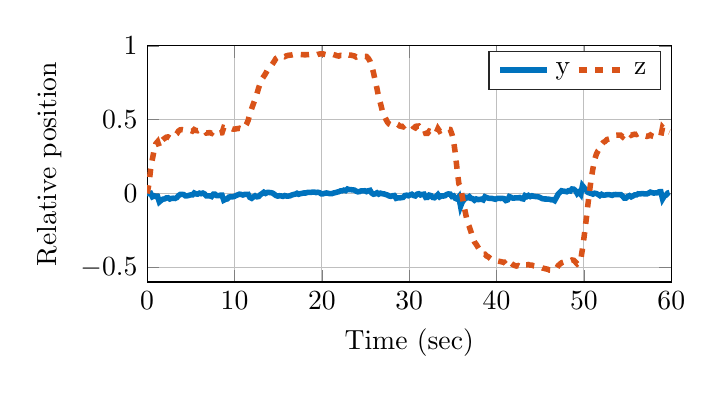
\begin{tikzpicture}

\begin{axis}[%
width=6.656442cm,
height=3cm,
at={(0cm,0cm)},
scale only axis,
xmin=0,
xmax=60,
xlabel={Time (sec)},
xmajorgrids,
ymin=-0.6,
ymax=1,
ylabel={Relative position},
ymajorgrids,
legend style={legend columns=2,legend cell align=left,align=left,draw=white!15!black}
]
\addplot [color=mycolor1,solid,line width=2.0pt]
  table[row sep=crcr]{%
0	0\\
0.199335548172757	-0.00132058126557062\\
0.398671096345515	0.00112234640962325\\
0.598006644518272	-0.0221758815843431\\
0.79734219269103	-0.0160516785955867\\
0.996677740863787	-0.0210493810476044\\
1.19601328903654	-0.0200937291681225\\
1.3953488372093	-0.0569547203691796\\
1.59468438538206	-0.0467111942385056\\
1.79401993355482	-0.0389397170264447\\
1.99335548172757	-0.0370453317726938\\
2.19269102990033	-0.0303027647712935\\
2.39202657807309	-0.0292933386008251\\
2.59136212624585	-0.0375077725539325\\
2.7906976744186	-0.0332072512836254\\
2.99003322259136	-0.0323534524585916\\
3.18936877076412	-0.033824258428504\\
3.38870431893688	-0.0283771891275158\\
3.58803986710963	-0.0147978995369406\\
3.78737541528239	-0.00660786899296631\\
3.98671096345515	-0.0060419580229141\\
4.18604651162791	-0.00755431526729347\\
4.38538205980066	-0.0165982746997833\\
4.58471760797342	-0.0157162112140435\\
4.78405315614618	-0.0129799995660891\\
4.98338870431894	-0.00977236771006398\\
5.18272425249169	-0.00981904394024732\\
5.38205980066445	0.0029179963557584\\
5.58139534883721	-0.00318178736703598\\
5.78073089700997	-0.00429637621803455\\
5.98006644518272	0.00199804309288718\\
6.17940199335548	-0.00159390967068679\\
6.37873754152824	0.00235728219300188\\
6.578073089701	-0.00367927957366479\\
6.77740863787375	-0.0165366532726649\\
6.97674418604651	-0.0165302627493666\\
7.17607973421927	-0.016311902994118\\
7.37541528239203	-0.0206215718840356\\
7.57475083056478	-0.00536735763458115\\
7.77408637873754	-0.00537012783925528\\
7.9734219269103	-0.0150186998199849\\
8.17275747508306	-0.0150931922164926\\
8.37209302325581	-0.0118806972916885\\
8.57142857142857	-0.0120375609373584\\
8.77076411960133	-0.0458311716202862\\
8.97009966777409	-0.0399878333222684\\
9.16943521594684	-0.0371217284279117\\
9.3687707641196	-0.0244092955571834\\
9.56810631229236	-0.0222749049566412\\
9.76744186046512	-0.0229425872149865\\
9.96677740863787	-0.0202392439595224\\
10.1661129568106	-0.0140213135729936\\
10.3654485049834	-0.00973655185574929\\
10.5647840531561	-0.0046491120687418\\
10.7641196013289	-0.00681133785406565\\
10.9634551495017	-0.0105151040348745\\
11.1627906976744	-0.00621382968049736\\
11.3621262458472	-0.00624339679834773\\
11.5614617940199	-0.00580286668085125\\
11.7607973421927	-0.0268853944347704\\
11.9601328903654	-0.0329362952087819\\
12.1594684385382	-0.0239727574082904\\
12.358803986711	-0.0159182634244992\\
12.5581395348837	-0.0227681298697363\\
12.7574750830565	-0.0209364188022035\\
12.9568106312292	-0.00842234932187419\\
13.156146179402	-0.000961887596118427\\
13.3554817275748	0.00811753484558908\\
13.5548172757475	0.000484981244953109\\
13.7541528239203	0.00650835708071373\\
13.953488372093	0.00668230581102663\\
14.1528239202658	0.00545102663100666\\
14.3521594684385	0.0028300068803806\\
14.5514950166113	-0.00543697383414987\\
14.7508305647841	-0.0142879813213174\\
14.9501661129568	-0.0179795595221858\\
15.1495016611296	-0.015190981256146\\
15.3488372093023	-0.0169191634930204\\
15.5481727574751	-0.0195227788484596\\
15.7475083056478	-0.0143830403286773\\
15.9468438538206	-0.0174095503597311\\
16.1461794019934	-0.0180256750898684\\
16.3455149501661	-0.0160617908740833\\
16.5448504983389	-0.0106333230915679\\
16.7441860465116	-0.00699286745503241\\
16.9435215946844	-0.00470905828378065\\
17.1428571428571	0.001202089406041\\
17.3421926910299	-0.00547231219600586\\
17.5415282392027	-0.00139578428045323\\
17.7408637873754	0.000762409726418722\\
17.9401993355482	0.00315775771642202\\
18.1395348837209	0.00299214049189495\\
18.3388704318937	0.00661424053910065\\
18.5382059800664	0.0066518236788824\\
18.7375415282392	0.00739808943883474\\
18.936877076412	0.0090108721874077\\
19.1362126245847	0.00947296990347396\\
19.3355481727575	0.00610680391003376\\
19.5348837209302	0.00797470600002337\\
19.734219269103	0.0054359357264902\\
19.9335548172757	-0.0023669702636947\\
20.1328903654485	-0.00215894241709758\\
20.3322259136213	0.00100179428796954\\
20.531561461794	0.00337420460168653\\
20.7308970099668	0.000970398114011173\\
20.9302325581395	-0.00165880504761673\\
21.1295681063123	-0.00169419008445382\\
21.3289036544851	0.00307194907039171\\
21.5282392026578	0.00539638484123339\\
21.7275747508306	0.00899387954303676\\
21.9269102990033	0.01151497933903\\
22.1262458471761	0.0172503944169504\\
22.3255813953488	0.0181585063445678\\
22.5249169435216	0.0225535667125698\\
22.7242524916944	0.0189040080853645\\
22.9235880398671	0.0298374035843634\\
23.1229235880399	0.0258960886186465\\
23.3222591362126	0.025531626594856\\
23.5215946843854	0.0243552227982798\\
23.7209302325581	0.022810531059698\\
23.9202657807309	0.0157030180788755\\
24.1196013289037	0.0111265043775438\\
24.3189368770764	0.0128673592228819\\
24.5182724252492	0.0179158265535845\\
24.7176079734219	0.0175609058222229\\
24.9169435215947	0.0183219969107925\\
25.1162790697674	0.0127320369797783\\
25.3156146179402	0.0182950004640497\\
25.514950166113	0.0210259655716238\\
25.7142857142857	0.00231044131957503\\
25.9136212624585	-0.00500694487227649\\
26.1129568106312	-0.00217510752693267\\
26.312292358804	0.00431840387233745\\
26.5116279069767	-0.00448819475381967\\
26.7109634551495	0.0017021526710983\\
26.9102990033223	-0.00163042837551197\\
27.109634551495	-0.00282936665146627\\
27.3089700996678	-0.00733613151461229\\
27.5083056478405	-0.010292680676175\\
27.7076411960133	-0.0172459171579233\\
27.906976744186	-0.0195290010692789\\
28.1063122923588	-0.0156275018501294\\
28.3056478405316	-0.0139917059958779\\
28.5049833887043	-0.0328515878248887\\
28.7043189368771	-0.0296400273065596\\
28.9036544850498	-0.0304513680860776\\
29.1029900332226	-0.0283534305557982\\
29.3023255813953	-0.0267063701359468\\
29.5016611295681	-0.0141552721390794\\
29.7009966777409	-0.0118064872731264\\
29.9003322259136	-0.0156432211977925\\
30.0996677740864	-0.0100617002186839\\
30.2990033222591	-0.00549787373956639\\
30.4983388704319	-0.01381204736786\\
30.6976744186047	-0.0168542459546999\\
30.8970099667774	-0.00463744358716067\\
31.0963455149502	-0.00210112153581635\\
31.2956810631229	-0.0102923114308223\\
31.4950166112957	-0.00639673305436064\\
31.6943521594684	-0.0048070320302103\\
31.8936877076412	-0.0272380729098439\\
32.093023255814	-0.0265326996393978\\
32.2923588039867	-0.0114683715671129\\
32.4916943521595	-0.0146480387607772\\
32.6910299003322	-0.026921931592385\\
32.890365448505	-0.0290567866946308\\
33.0897009966777	-0.0202172940201026\\
33.2890365448505	-0.00759016160020315\\
33.4883720930233	-0.0231027454134682\\
33.687707641196	-0.0164410692431156\\
33.8870431893688	-0.0175544037358568\\
34.0863787375415	-0.0154757491532584\\
34.2857142857143	-0.00675030915932379\\
34.485049833887	-0.00321491640880095\\
34.6843853820598	-0.0044683930990948\\
34.8837209302326	-0.0202450509298384\\
35.0830564784053	-0.0166770721159805\\
35.2823920265781	-0.0331777048389378\\
35.4817275747508	-0.0382038422492392\\
35.6810631229236	-0.0233914689040189\\
35.8803986710963	-0.0871536978997415\\
36.0797342192691	-0.0568451183871289\\
36.2790697674419	-0.0427287008190841\\
36.4784053156146	-0.0260746956697238\\
36.6777408637874	-0.0292301620887247\\
36.8770764119601	-0.0215854792985424\\
37.0764119601329	-0.0335358923563557\\
37.2757475083056	-0.0355738182517397\\
37.4750830564784	-0.0458712537646057\\
37.6744186046512	-0.0374633068741393\\
37.8737541528239	-0.041106255929872\\
38.0730897009967	-0.0407540591835303\\
38.2724252491694	-0.0383105726889664\\
38.4717607973422	-0.043526190694328\\
38.671096345515	-0.0227870212626\\
38.8704318936877	-0.0281441983782241\\
39.0697674418605	-0.0321823791774265\\
39.2691029900332	-0.0333582742687662\\
39.468438538206	-0.0336331263934739\\
39.6677740863787	-0.0366558036196255\\
39.8671096345515	-0.0393343624989057\\
40.0664451827243	-0.0340759215317715\\
40.265780730897	-0.033073871388856\\
40.4651162790698	-0.0340924436737625\\
40.6644518272425	-0.0335566757241526\\
40.8637873754153	-0.0353352088812731\\
41.063122923588	-0.0475973204235304\\
41.2624584717608	-0.0437769524488301\\
41.4617940199336	-0.0214467287136847\\
41.6611295681063	-0.0258762729230209\\
41.8604651162791	-0.0316644741933116\\
42.0598006644518	-0.0307653284372013\\
42.2591362126246	-0.0304424438485263\\
42.4584717607973	-0.0301816307780778\\
42.6578073089701	-0.0277326249448472\\
42.8571428571429	-0.0347070898469835\\
43.0564784053156	-0.0370354521544376\\
43.2558139534884	-0.0152223717069049\\
43.4551495016611	-0.0216608935689415\\
43.6544850498339	-0.0136574094475869\\
43.8538205980066	-0.0208931713585512\\
44.0531561461794	-0.0156116751016013\\
44.2524916943522	-0.0189003512065203\\
44.4518272425249	-0.0209334612817265\\
44.6511627906977	-0.0214575100913635\\
44.8504983388704	-0.0238221008592978\\
45.0498338870432	-0.0298586651645122\\
45.2491694352159	-0.0352443610835564\\
45.4485049833887	-0.037427577828785\\
45.6478405315615	-0.0375160189179315\\
45.8471760797342	-0.0379301679332619\\
46.046511627907	-0.0394297329859675\\
46.2458471760797	-0.042667960447993\\
46.4451827242525	-0.0419613748354148\\
46.6445182724253	-0.0485856690026544\\
46.843853820598	-0.0279369614529532\\
47.0431893687708	-0.00498054926770558\\
47.2425249169435	0.00721056556783473\\
47.4418604651163	0.0181972697769673\\
47.641196013289	0.0151518115118004\\
47.8405315614618	0.0147059479993652\\
48.0398671096346	0.0115872235616521\\
48.2392026578073	0.01873715423679\\
48.4385382059801	0.0164013166910819\\
48.6378737541528	0.0301403378384373\\
48.8372093023256	0.0288206118045925\\
49.0365448504983	0.0186980752397817\\
49.2358803986711	-0.00112410669663085\\
49.4352159468439	0.00956883902144773\\
49.6345514950166	-0.00543048446200062\\
49.8338870431894	0.0523928732189702\\
50.0332225913621	0.0379312767683394\\
50.2325581395349	0.0244197905429689\\
50.4318936877076	0.00822977071636547\\
50.6312292358804	0.00309696391732872\\
50.8305647840532	5.66517215710785e-05\\
51.0299003322259	-0.00450712691600763\\
51.2292358803987	0.00146737653537179\\
51.4285714285714	-0.000629590910142336\\
51.6279069767442	-0.00651224981098017\\
51.8272425249169	-0.0146560747101482\\
52.0265780730897	-0.00581593537941441\\
52.2259136212625	-0.0118053033398487\\
52.4252491694352	-0.0108278864724125\\
52.624584717608	-0.00855674811747609\\
52.8239202657807	-0.0079369996930885\\
53.0232558139535	-0.00941891089286701\\
53.2225913621263	-0.0128491791158026\\
53.421926910299	-0.00846457623990035\\
53.6212624584718	-0.00716090854116988\\
53.8205980066445	-0.00727855752603926\\
54.0199335548173	-0.00749034243172436\\
54.21926910299	-0.00734008385871468\\
54.4186046511628	-0.0176699226279297\\
54.6179401993356	-0.0313607070322785\\
54.8172757475083	-0.0310163073846977\\
55.0166112956811	-0.020247387987544\\
55.2159468438538	-0.0148998124574308\\
55.4152823920266	-0.0228306491637155\\
55.6146179401993	-0.0170163327972076\\
55.8139534883721	-0.00972925026365587\\
56.0132890365449	-0.00978971144278848\\
56.2126245847176	-0.00226422983901356\\
56.4119601328904	-0.00294907204492753\\
56.6112956810631	-0.00132338574438154\\
56.8106312292359	-0.00156711780720925\\
57.0099667774086	-0.00349074886248438\\
57.2093023255814	-0.00321795781158943\\
57.4086378737542	0.00200332672661796\\
57.6079734219269	0.00887331944002981\\
57.8073089700997	0.00512301539777399\\
58.0066445182724	0.002718835214434\\
58.2059800664452	0.00352097815064242\\
58.4053156146179	0.00471708418672223\\
58.6046511627907	0.0112949906383608\\
58.8039867109635	0.0118616474893772\\
59.0033222591362	-0.0370111635557219\\
59.202657807309	-0.0176573203030217\\
59.4019933554817	-0.0113347875574306\\
59.6013289036545	0.00268585240987218\\
59.8006644518272	0.00664434792096072\\
};
\addlegendentry{y};

\addplot [color=mycolor2,dashed,line width=2.0pt]
  table[row sep=crcr]{%
0	0\\
0.199335548172757	0.0628046371175146\\
0.398671096345515	0.164624715018646\\
0.598006644518272	0.232338525235059\\
0.79734219269103	0.293704510130543\\
0.996677740863787	0.337073745808173\\
1.19601328903654	0.350730403111273\\
1.3953488372093	0.31647309567279\\
1.59468438538206	0.353633313384843\\
1.79401993355482	0.363878191412139\\
1.99335548172757	0.372823656800767\\
2.19269102990033	0.381030588021011\\
2.39202657807309	0.382889379802406\\
2.59136212624585	0.375601726072534\\
2.7906976744186	0.389283406756786\\
2.99003322259136	0.389656294687813\\
3.18936877076412	0.394930586914796\\
3.38870431893688	0.403798199330499\\
3.58803986710963	0.422879970493739\\
3.78737541528239	0.430966772819947\\
3.98671096345515	0.432158948711074\\
4.18604651162791	0.430103169324368\\
4.38538205980066	0.433185514727501\\
4.58471760797342	0.432451884444823\\
4.78405315614618	0.430237289248159\\
4.98338870431894	0.426510815513719\\
5.18272425249169	0.42212738152349\\
5.38205980066445	0.432656948921522\\
5.58139534883721	0.426483685602419\\
5.78073089700997	0.424744456748277\\
5.98006644518272	0.430635317271265\\
6.17940199335548	0.427162999392397\\
6.37873754152824	0.429970302232517\\
6.578073089701	0.423855139419677\\
6.77740863787375	0.409166879017323\\
6.97674418604651	0.410741277667944\\
7.17607973421927	0.411924047370872\\
7.37541528239203	0.407368848210361\\
7.57475083056478	0.421505556551943\\
7.77408637873754	0.421439715465597\\
7.9734219269103	0.41149946260234\\
8.17275747508306	0.406463635886945\\
8.37209302325581	0.409704619118764\\
8.57142857142857	0.410923777525318\\
8.77076411960133	0.446446232959511\\
8.97009966777409	0.442854281034078\\
9.16943521594684	0.438339479865388\\
9.3687707641196	0.443817344037112\\
9.56810631229236	0.441547325870856\\
9.76744186046512	0.43683272107882\\
9.96677740863787	0.435362574022963\\
10.1661129568106	0.437670718062059\\
10.3654485049834	0.439196025118962\\
10.5647840531561	0.441542373820451\\
10.7641196013289	0.437709987370259\\
10.9634551495017	0.435166923819941\\
11.1627906976744	0.44846809560248\\
11.3621262458472	0.467668674141722\\
11.5614617940199	0.494671543881253\\
11.7607973421927	0.540171617425558\\
11.9601328903654	0.574363957275514\\
12.1594684385382	0.606925090461892\\
12.358803986711	0.637436789059091\\
12.5581395348837	0.672473810423877\\
12.7574750830565	0.714120522469777\\
12.9568106312292	0.747889569475743\\
13.156146179402	0.776113342694485\\
13.3554817275748	0.793142900900466\\
13.5548172757475	0.811638925129972\\
13.7541528239203	0.833910320174686\\
13.953488372093	0.845534869694772\\
14.1528239202658	0.860640486212742\\
14.3521594684385	0.877323800619262\\
14.5514950166113	0.895069626570558\\
14.7508305647841	0.914785041210788\\
14.9501661129568	0.922045250253588\\
15.1495016611296	0.928595918429915\\
15.3488372093023	0.932362265665065\\
15.5481727574751	0.932476669811816\\
15.7475083056478	0.926839804645889\\
15.9468438538206	0.932112614869322\\
16.1461794019934	0.935772458784624\\
16.3455149501661	0.936373639958059\\
16.5448504983389	0.938306679717779\\
16.7441860465116	0.941171159249652\\
16.9435215946844	0.93916779945567\\
17.1428571428571	0.936426699190952\\
17.3421926910299	0.939775362715449\\
17.5415282392027	0.941380035674384\\
17.7408637873754	0.940213897395907\\
17.9401993355482	0.939518809605958\\
18.1395348837209	0.939435070406905\\
18.3388704318937	0.939781664380064\\
18.5382059800664	0.940971796799975\\
18.7375415282392	0.940045772804738\\
18.936877076412	0.939601372930136\\
19.1362126245847	0.938065510462054\\
19.3355481727575	0.937509100846976\\
19.5348837209302	0.942176014221331\\
19.734219269103	0.944343775275839\\
19.9335548172757	0.945874414454823\\
20.1328903654485	0.945582378345532\\
20.3322259136213	0.941867180156399\\
20.531561461794	0.938988080029339\\
20.7308970099668	0.941677875416307\\
20.9302325581395	0.944977561566657\\
21.1295681063123	0.94485266756232\\
21.3289036544851	0.940226481398062\\
21.5282392026578	0.937449118606303\\
21.7275747508306	0.933134853540975\\
21.9269102990033	0.930839190121693\\
22.1262458471761	0.935096809888216\\
22.3255813953488	0.934476048987226\\
22.5249169435216	0.930384395450076\\
22.7242524916944	0.93087697589798\\
22.9235880398671	0.941507378258433\\
23.1229235880399	0.937385522388138\\
23.3222591362126	0.937079796043526\\
23.5215946843854	0.933848560065183\\
23.7209302325581	0.93163484823172\\
23.9202657807309	0.924208698543224\\
24.1196013289037	0.929159842753192\\
24.3189368770764	0.929840416926988\\
24.5182724252492	0.931425871939374\\
24.7176079734219	0.930869059243131\\
24.9169435215947	0.92829646873974\\
25.1162790697674	0.927697682096421\\
25.3156146179402	0.914952369818018\\
25.514950166113	0.895842232045821\\
25.7142857142857	0.861533825794182\\
25.9136212624585	0.81708067691627\\
26.1129568106312	0.762975012912914\\
26.312292358804	0.709344688294075\\
26.5116279069767	0.648889509380146\\
26.7109634551495	0.609926447261129\\
26.9102990033223	0.56242014133315\\
27.109634551495	0.530393063233917\\
27.3089700996678	0.505247160731787\\
27.5083056478405	0.482906375926632\\
27.7076411960133	0.469808992121467\\
27.906976744186	0.464051742195728\\
28.1063122923588	0.465069547262159\\
28.3056478405316	0.463522372919038\\
28.5049833887043	0.472257171685205\\
28.7043189368771	0.466918277805492\\
28.9036544850498	0.456921946053901\\
29.1029900332226	0.454180181532397\\
29.3023255813953	0.451269905288428\\
29.5016611295681	0.461756340403109\\
29.7009966777409	0.465609699791755\\
29.9003322259136	0.45908803383052\\
30.0996677740864	0.461467279090852\\
30.2990033222591	0.462927811455594\\
30.4983388704319	0.450609596332786\\
30.6976744186047	0.444458367358376\\
30.8970099667774	0.456332065301771\\
31.0963455149502	0.456793528257051\\
31.2956810631229	0.443673406410546\\
31.4950166112957	0.439502058653878\\
31.6943521594684	0.440147753469679\\
31.8936877076412	0.407237308071256\\
32.093023255814	0.406946566223137\\
32.2923588039867	0.422100549895473\\
32.4916943521595	0.418152268314429\\
32.6910299003322	0.405025866664081\\
32.890365448505	0.401861260115696\\
33.0897009966777	0.41066384002224\\
33.2890365448505	0.438667707571663\\
33.4883720930233	0.421313915549871\\
33.687707641196	0.427102007423966\\
33.8870431893688	0.422179411992096\\
34.0863787375415	0.424106346619788\\
34.2857142857143	0.43283745396059\\
34.485049833887	0.435977248191426\\
34.6843853820598	0.433145018135297\\
34.8837209302326	0.402028742440632\\
35.0830564784053	0.354767848375029\\
35.2823920265781	0.26911781710107\\
35.4817275747508	0.161828276106424\\
35.6810631229236	0.0659699371070213\\
35.8803986710963	0.0439911963071715\\
36.0797342192691	-0.0246805623952793\\
36.2790697674419	-0.0860244167892457\\
36.4784053156146	-0.143068106773873\\
36.6777408637874	-0.199533642301228\\
36.8770764119601	-0.224803444768662\\
37.0764119601329	-0.260984715722745\\
37.2757475083056	-0.300931425453161\\
37.4750830564784	-0.329243429464966\\
37.6744186046512	-0.34501555512092\\
37.8737541528239	-0.364249505349367\\
38.0730897009967	-0.382884570965979\\
38.2724252491694	-0.397245445682436\\
38.4717607973422	-0.412754293255826\\
38.671096345515	-0.411714168138778\\
38.8704318936877	-0.424069878684422\\
39.0697674418605	-0.429844190755993\\
39.2691029900332	-0.439674534449786\\
39.468438538206	-0.448517508679879\\
39.6677740863787	-0.453241644092873\\
39.8671096345515	-0.455175901884305\\
40.0664451827243	-0.456831708008758\\
40.265780730897	-0.459278457665809\\
40.4651162790698	-0.461552306882504\\
40.6644518272425	-0.464554785131151\\
40.8637873754153	-0.464845651453576\\
41.063122923588	-0.478436975440131\\
41.2624584717608	-0.483550701826827\\
41.4617940199336	-0.464149430878842\\
41.6611295681063	-0.472514603825698\\
41.8604651162791	-0.481452532728842\\
42.0598006644518	-0.487935082951695\\
42.2591362126246	-0.491270742559196\\
42.4584717607973	-0.488556737394788\\
42.6578073089701	-0.493961461038429\\
42.8571428571429	-0.497005069814619\\
43.0564784053156	-0.498783534563381\\
43.2558139534884	-0.484031809305319\\
43.4551495016611	-0.483601588595119\\
43.6544850498339	-0.481694897685294\\
43.8538205980066	-0.485782419779176\\
44.0531561461794	-0.486015964783104\\
44.2524916943522	-0.490107567834349\\
44.4518272425249	-0.492188332694897\\
44.6511627906977	-0.492420739523374\\
44.8504983388704	-0.497466291664849\\
45.0498338870432	-0.499493320294128\\
45.2491694352159	-0.50487577440312\\
45.4485049833887	-0.50764750589163\\
45.6478405315615	-0.51094263518841\\
45.8471760797342	-0.513161182163215\\
46.046511627907	-0.518829026960023\\
46.2458471760797	-0.519729279534146\\
46.4451827242525	-0.520706389036425\\
46.6445182724253	-0.520746783365489\\
46.843853820598	-0.510121770298556\\
47.0431893687708	-0.489634050673141\\
47.2425249169435	-0.478706703871641\\
47.4418604651163	-0.469628285107495\\
47.641196013289	-0.465628070872782\\
47.8405315614618	-0.465572460746791\\
48.0398671096346	-0.462267019765786\\
48.2392026578073	-0.453295727181728\\
48.4385382059801	-0.455417673681622\\
48.6378737541528	-0.450824019246657\\
48.8372093023256	-0.452909508739999\\
49.0365448504983	-0.464638576622007\\
49.2358803986711	-0.477435572228638\\
49.4352159468439	-0.468466057546884\\
49.6345514950166	-0.449988744094738\\
49.8338870431894	-0.375036169402439\\
50.0332225913621	-0.28798165620689\\
50.2325581395349	-0.191738256251821\\
50.4318936877076	-0.087955240325692\\
50.6312292358804	0.0097935082244934\\
50.8305647840532	0.0977976021257687\\
51.0299003322259	0.168093822841909\\
51.2292358803987	0.231455436071317\\
51.4285714285714	0.266914454664858\\
51.6279069767442	0.289887468363336\\
51.8272425249169	0.30193779291444\\
52.0265780730897	0.332349104275859\\
52.2259136212625	0.346222939162992\\
52.4252491694352	0.352301740754296\\
52.624584717608	0.364824634916193\\
52.8239202657807	0.368059338658299\\
53.0232558139535	0.37127463068562\\
53.2225913621263	0.376718041222536\\
53.421926910299	0.384479049723518\\
53.6212624584718	0.393819092071035\\
53.8205980066445	0.394708982348069\\
54.0199335548173	0.394391899430323\\
54.21926910299	0.394418377167806\\
54.4186046511628	0.384127517148574\\
54.6179401993356	0.398703266799899\\
54.8172757475083	0.395426007399552\\
55.0166112956811	0.405156806793236\\
55.2159468438538	0.406273019098515\\
55.4152823920266	0.394200108886405\\
55.6146179401993	0.39875574019461\\
55.8139534883721	0.401017817083248\\
56.0132890365449	0.399022326243276\\
56.2126245847176	0.40531696770714\\
56.4119601328904	0.401052396043522\\
56.6112956810631	0.398564942083973\\
56.8106312292359	0.395018183650631\\
57.0099667774086	0.38953085280502\\
57.2093023255814	0.386517921440947\\
57.4086378737542	0.389762235216575\\
57.6079734219269	0.396342438224218\\
57.8073089700997	0.388905790281216\\
58.0066445182724	0.385430620155106\\
58.2059800664452	0.385727876703996\\
58.4053156146179	0.384145039388635\\
58.6046511627907	0.389311875337958\\
58.8039867109635	0.3889454440519\\
59.0033222591362	0.447199695223942\\
59.202657807309	0.433740337486534\\
59.4019933554817	0.422542727491619\\
59.6013289036545	0.420791511609495\\
59.8006644518272	0.416154987607728\\
};
\addlegendentry{z};

\end{axis}
\end{tikzpicture}%
      \label{fig:XYcentre}
      \caption{Relative position} 
      %Cross product between principal lines of a corridor, (b)
      %    relative position between the cross product and the principal lines }
    \label{fig:centrePosition}
  \end{figure}



  \begin{figure}[!h]
  \centering
     % This file was created by matlab2tikz.
% Minimal pgfplots version: 1.3
%
%The latest updates can be retrieved from
%  http://www.mathworks.com/matlabcentral/fileexchange/22022-matlab2tikz
%where you can also make suggestions and rate matlab2tikz.
%
\definecolor{mycolor1}{rgb}{0.00000,0.44700,0.74100}%
\definecolor{mycolor2}{rgb}{0.85000,0.32500,0.09800}%
%
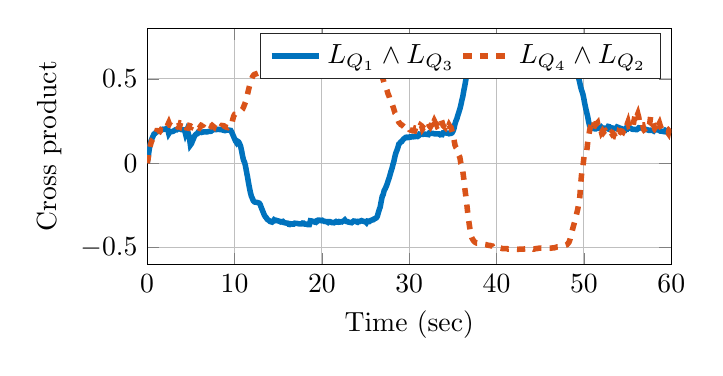
\begin{tikzpicture}

\begin{axis}[%
width=6.656442cm,
height=3cm,
at={(0cm,0cm)},
scale only axis,
xmin=0,
xmax=60,
xlabel={Time (sec)},
xmajorgrids,
ymin=-0.6,
ymax=0.8,
ylabel={Cross product},
ymajorgrids,
legend style={legend columns=2,legend cell align=left,align=left,draw=white!15!black}
]
\addplot [color=mycolor1,solid,line width=2.0pt]
  table[row sep=crcr]{%
0	0\\
0.112570356472795	0.0338128800506108\\
0.225140712945591	0.0781186744950125\\
0.337711069418386	0.112470076980368\\
0.450281425891182	0.132880043941261\\
0.562851782363977	0.147437189653863\\
0.675422138836773	0.159909831886464\\
0.787992495309569	0.173379750236549\\
0.900562851782364	0.176264102408247\\
1.01313320825516	0.183582430962678\\
1.12570356472796	0.185493038872155\\
1.23827392120075	0.188500038723374\\
1.35084427767355	0.190757784253662\\
1.46341463414634	0.192834868892969\\
1.57598499061914	0.19535092246597\\
1.68855534709193	0.198432278513121\\
1.80112570356473	0.201207350660654\\
1.91369606003752	0.200596821078583\\
2.02626641651032	0.202248958838729\\
2.13883677298311	0.203659268707712\\
2.25140712945591	0.202816675813975\\
2.36397748592871	0.199219959979387\\
2.4765478424015	0.175936345472609\\
2.5891181988743	0.185040916768287\\
2.70168855534709	0.185979765787084\\
2.81425891181989	0.187603916497351\\
2.92682926829268	0.188156860363543\\
3.03939962476548	0.191394924233384\\
3.15196998123827	0.195114673020982\\
3.26454033771107	0.198582073235385\\
3.37711069418386	0.197773574842031\\
3.48968105065666	0.202474498424629\\
3.60225140712946	0.204347951411614\\
3.71482176360225	0.204103882431725\\
3.82739212007505	0.201469844139015\\
3.93996247654784	0.199175983698453\\
4.05253283302064	0.199035397348986\\
4.16510318949343	0.197312338183083\\
4.27767354596623	0.197355204038733\\
4.39024390243902	0.1745236750114\\
4.50281425891182	0.189318337076791\\
4.61538461538462	0.17032913994802\\
4.72795497185741	0.171684279037693\\
4.84052532833021	0.149493974199423\\
4.953095684803	0.108024014169737\\
5.0656660412758	0.115930416531766\\
5.17823639774859	0.130531388958703\\
5.29080675422139	0.144264355232999\\
5.40337711069418	0.158969251197829\\
5.51594746716698	0.167402025625788\\
5.62851782363977	0.172996645383662\\
5.74108818011257	0.174511554553017\\
5.85365853658537	0.184626951755902\\
5.96622889305816	0.18501233345537\\
6.07879924953096	0.182249372162074\\
6.19136960600375	0.182089897531924\\
6.30393996247655	0.183511208914705\\
6.41651031894934	0.185243880849872\\
6.52908067542214	0.185174086269186\\
6.64165103189493	0.185892012121156\\
6.75422138836773	0.185136355308999\\
6.86679174484053	0.1854975225442\\
6.97936210131332	0.187689967445412\\
7.09193245778612	0.188248588834192\\
7.20450281425891	0.188267238440533\\
7.31707317073171	0.189672437281292\\
7.4296435272045	0.194677394294628\\
7.5422138836773	0.198036549251512\\
7.65478424015009	0.199371017368896\\
7.76735459662289	0.199204868894711\\
7.87992495309569	0.199610178048138\\
7.99249530956848	0.19986646729688\\
8.10506566604128	0.199980617281622\\
8.21763602251407	0.200190177853059\\
8.33020637898687	0.199624481841326\\
8.44277673545966	0.198827634361661\\
8.55534709193246	0.198117108518734\\
8.66791744840525	0.196295468947635\\
8.78048780487805	0.194612752600557\\
8.89305816135084	0.193562503686751\\
9.00562851782364	0.193969562205689\\
9.11819887429644	0.197058721199376\\
9.23076923076923	0.19689883343058\\
9.34333958724203	0.195955917780991\\
9.45590994371482	0.195415796610041\\
9.56848030018762	0.194154713132345\\
9.68105065666041	0.183524860957425\\
9.79362101313321	0.170615761678194\\
9.906191369606	0.15674780880419\\
10.0187617260788	0.14321488878955\\
10.1313320825516	0.130298995433052\\
10.2439024390244	0.12166528304015\\
10.3564727954972	0.129892187829227\\
10.46904315197	0.126276044222144\\
10.5816135084428	0.115543593149062\\
10.6941838649156	0.100898330963019\\
10.8067542213884	0.0752984212686885\\
10.9193245778612	0.0434736503976224\\
11.031894934334	0.0179384503236599\\
11.1444652908068	0.00684359180763483\\
11.2570356472795	-0.0166869582439842\\
11.3696060037523	-0.0488978468835196\\
11.4821763602251	-0.0790104774474624\\
11.5947467166979	-0.113460974646368\\
11.7073170731707	-0.144891511637877\\
11.8198874296435	-0.173675131912444\\
11.9324577861163	-0.196181593293089\\
12.0450281425891	-0.208206175999706\\
12.1575984990619	-0.223231254887624\\
12.2701688555347	-0.229213882208691\\
12.3827392120075	-0.23101896821864\\
12.4953095684803	-0.231633399722565\\
12.6078799249531	-0.232942180794323\\
12.7204502814259	-0.234419318338329\\
12.8330206378987	-0.236965710848388\\
12.9455909943715	-0.244957745891395\\
13.0581613508443	-0.261954917533339\\
13.1707317073171	-0.276235335972997\\
13.2833020637899	-0.290182449686313\\
13.3958724202627	-0.305245212501116\\
13.5084427767355	-0.315917035254263\\
13.6210131332083	-0.321862884100609\\
13.7335834896811	-0.331724989360136\\
13.8461538461538	-0.335702913467911\\
13.9587242026266	-0.340468243383304\\
14.0712945590994	-0.345478233851735\\
14.1838649155722	-0.347470559274428\\
14.296435272045	-0.34896713408192\\
14.4090056285178	-0.34366991121753\\
14.5215759849906	-0.335926528894775\\
14.6341463414634	-0.340209170136963\\
14.7467166979362	-0.338242156919721\\
14.859287054409	-0.340042357908668\\
14.9718574108818	-0.341789240477192\\
15.0844277673546	-0.342848186180256\\
15.1969981238274	-0.346125879006961\\
15.3095684803002	-0.34841524676692\\
15.422138836773	-0.346402447421877\\
15.5347091932458	-0.34497771274764\\
15.6472795497186	-0.351484523264604\\
15.7598499061914	-0.353088436210777\\
15.8724202626642	-0.354081653556549\\
15.984990619137	-0.355207416008695\\
16.0975609756098	-0.355670345840297\\
16.2101313320826	-0.362120933313116\\
16.3227016885553	-0.363209402084913\\
16.4352720450281	-0.358920606602676\\
16.5478424015009	-0.359185967770079\\
16.6604127579737	-0.360882789860906\\
16.7729831144465	-0.360642828853224\\
16.8855534709193	-0.355568034809691\\
16.9981238273921	-0.356160247906048\\
17.1106941838649	-0.356741233912473\\
17.2232645403377	-0.357562503190737\\
17.3358348968105	-0.358747514232504\\
17.4484052532833	-0.359011843877269\\
17.5609756097561	-0.359316768095886\\
17.6735459662289	-0.359003782865682\\
17.7861163227017	-0.354545162995028\\
17.8986866791745	-0.354890589751355\\
18.0112570356473	-0.360288171328559\\
18.1238273921201	-0.360852043971566\\
18.2363977485929	-0.360985178149573\\
18.3489681050657	-0.363226570179795\\
18.4615384615385	-0.363235914046092\\
18.5741088180113	-0.363205993257601\\
18.6866791744841	-0.341237034247378\\
18.7992495309568	-0.342154297686383\\
18.9118198874296	-0.343818887012021\\
19.0243902439024	-0.345198996795264\\
19.1369606003752	-0.348085869497819\\
19.249530956848	-0.344719225527737\\
19.3621013133208	-0.349007938270244\\
19.4746716697936	-0.344609653888941\\
19.5872420262664	-0.337289038874431\\
19.6998123827392	-0.337032802799652\\
19.812382739212	-0.33914523396219\\
19.9249530956848	-0.340600006821824\\
20.0375234521576	-0.338398094348933\\
20.1500938086304	-0.341453196718409\\
20.2626641651032	-0.344614511266779\\
20.375234521576	-0.345004581286897\\
20.4878048780488	-0.346661977793001\\
20.6003752345216	-0.346947549565181\\
20.7129455909944	-0.351003380233841\\
20.8255159474672	-0.346330481873011\\
20.93808630394	-0.346695000169738\\
21.0506566604128	-0.348643828177225\\
21.1632270168856	-0.35237063987166\\
21.2757973733583	-0.352442708352689\\
21.3883677298311	-0.35289343043788\\
21.5009380863039	-0.348782115684998\\
21.6135084427767	-0.345641878372057\\
21.7260787992495	-0.349218992514277\\
21.8386491557223	-0.349734389205368\\
21.9512195121951	-0.346298445657587\\
22.0637898686679	-0.348816683626059\\
22.1763602251407	-0.347219031851382\\
22.2889305816135	-0.347986442206714\\
22.4015009380863	-0.344199722332578\\
22.5140712945591	-0.341460413232574\\
22.6266416510319	-0.336259690791491\\
22.7392120075047	-0.343464837120666\\
22.8517823639775	-0.346028898286896\\
22.9643527204503	-0.346258307065097\\
23.0769230769231	-0.34953162376588\\
23.1894934333959	-0.350241054558031\\
23.3020637898687	-0.351316245400566\\
23.4146341463415	-0.352497011942653\\
23.5272045028143	-0.347671546461057\\
23.6397748592871	-0.342617639371094\\
23.7523452157598	-0.343029736085272\\
23.8649155722326	-0.344483831815534\\
23.9774859287054	-0.347640554122646\\
24.0900562851782	-0.349689206489917\\
24.202626641651	-0.344791174482075\\
24.3151969981238	-0.34564744588621\\
24.4277673545966	-0.342351130085401\\
24.5403377110694	-0.340260302304975\\
24.6529080675422	-0.342762866620129\\
24.765478424015	-0.344314959039089\\
24.8780487804878	-0.346107829548641\\
24.9906191369606	-0.346880731264235\\
25.1031894934334	-0.352571839209339\\
25.2157598499062	-0.343072893611689\\
25.328330206379	-0.344189016456062\\
25.4409005628518	-0.345250491054665\\
25.5534709193246	-0.340077172882274\\
25.6660412757974	-0.338275167130577\\
25.7786116322702	-0.335608052232043\\
25.891181988743	-0.335101006120062\\
26.0037523452158	-0.329638678981123\\
26.1163227016886	-0.327431828060283\\
26.2288930581614	-0.323977163032604\\
26.3414634146341	-0.315628600429944\\
26.4540337711069	-0.295280024428115\\
26.5666041275797	-0.275598696081093\\
26.6791744840525	-0.259332198939687\\
26.7917448405253	-0.226680280754306\\
26.9043151969981	-0.1975320229684\\
27.0168855534709	-0.185981955139726\\
27.1294559099437	-0.162452854043388\\
27.2420262664165	-0.15208336516127\\
27.3545966228893	-0.139117280974921\\
27.4671669793621	-0.124275110901685\\
27.5797373358349	-0.105444378458061\\
27.6923076923077	-0.0896843737050856\\
27.8048780487805	-0.069250142715357\\
27.9174484052533	-0.0481793684088378\\
28.0300187617261	-0.0303655282016061\\
28.1425891181989	-0.00690468514111643\\
28.2551594746717	0.0128808865126376\\
28.3677298311445	0.0405438014661307\\
28.4803001876173	0.0620085656997668\\
28.5928705440901	0.0765116024942797\\
28.7054409005629	0.0937958491219562\\
28.8180112570356	0.113745993654071\\
28.9305816135084	0.119243920082785\\
29.0431519699812	0.126753999997576\\
29.155722326454	0.129261150206949\\
29.2682926829268	0.138366219858979\\
29.3808630393996	0.144547739767189\\
29.4934333958724	0.148403243517159\\
29.6060037523452	0.153348557010923\\
29.718574108818	0.154287075742953\\
29.8311444652908	0.151799141771775\\
29.9437148217636	0.152726033185129\\
30.0562851782364	0.155558380068955\\
30.1688555347092	0.154336987721779\\
30.281425891182	0.157054523984667\\
30.3939962476548	0.156924228076865\\
30.5065666041276	0.15676170448608\\
30.6191369606004	0.157105124356166\\
30.7317073170732	0.158503567499627\\
30.844277673546	0.158446652223626\\
30.9568480300188	0.158312012356577\\
31.0694183864916	0.162306110103494\\
31.1819887429644	0.172382553941931\\
31.2945590994372	0.171402432848205\\
31.4071294559099	0.171300957776138\\
31.5196998123827	0.175408798990629\\
31.6322701688555	0.171545112447451\\
31.7448405253283	0.172069724024796\\
31.8574108818011	0.171841952135441\\
31.9699812382739	0.171442630916486\\
32.0825515947467	0.170881744443728\\
32.1951219512195	0.169616246453653\\
32.3076923076923	0.179189359460962\\
32.4202626641651	0.178865987199561\\
32.5328330206379	0.176639461854871\\
32.6454033771107	0.176627860572761\\
32.7579737335835	0.176238519542516\\
32.8705440900563	0.174473720180308\\
32.9831144465291	0.173824499648275\\
33.0956848030019	0.173800955902285\\
33.2082551594747	0.173856563101419\\
33.3208255159475	0.173777994572302\\
33.4333958724203	0.173364179099412\\
33.5459662288931	0.168469752813557\\
33.6585365853659	0.169613336158769\\
33.7711069418387	0.169170627767453\\
33.8836772983114	0.179798481381829\\
33.9962476547842	0.179580203699488\\
34.108818011257	0.179967236272093\\
34.2213883677298	0.178871134162049\\
34.3339587242026	0.178293931606216\\
34.4465290806754	0.177816983722728\\
34.5590994371482	0.174659337261943\\
34.671669793621	0.176453938261385\\
34.7842401500938	0.176676214175266\\
34.8968105065666	0.179962010283622\\
35.0093808630394	0.189508245123292\\
35.1219512195122	0.204870814595846\\
35.234521575985	0.232452404166479\\
35.3470919324578	0.250471636428545\\
35.4596622889306	0.264237370122911\\
35.5722326454034	0.284733703236684\\
35.6848030018762	0.302552340726468\\
35.797373358349	0.321420526939557\\
35.9099437148218	0.344572455406793\\
36.0225140712946	0.37156912502672\\
36.1350844277674	0.395755462131469\\
36.2476547842402	0.429033471012503\\
36.3602251407129	0.458026221032905\\
36.4727954971857	0.491122438499188\\
36.5853658536585	0.530039874304947\\
36.6979362101313	0.563320125002019\\
36.8105065666041	0.600066310009515\\
36.9230769230769	0.630518057333651\\
37.0356472795497	0.652782451734124\\
37.1482176360225	0.677421877653545\\
37.2607879924953	0.686005913667979\\
37.3733583489681	0.69302879732752\\
37.4859287054409	0.693525255354537\\
37.5984990619137	0.695120901303095\\
37.7110694183865	0.698562446922637\\
37.8236397748593	0.698781458699101\\
37.9362101313321	0.699911771413797\\
38.0487804878049	0.700447108629663\\
38.1613508442777	0.701226408841879\\
38.2739212007505	0.701761984976572\\
38.3864915572233	0.701989260062872\\
38.4990619136961	0.702755134118271\\
38.6116322701689	0.703643281767371\\
38.7242026266417	0.704655138403564\\
38.8367729831145	0.70492714903003\\
38.9493433395872	0.705567682878607\\
39.06191369606	0.705853856050391\\
39.1744840525328	0.706684497729728\\
39.2870544090056	0.706698055125714\\
39.3996247654784	0.706719181273706\\
39.5121951219512	0.707534908043219\\
39.624765478424	0.708487339239622\\
39.7373358348968	0.70865540398382\\
39.8499061913696	0.709548041906067\\
39.9624765478424	0.709832306130323\\
40.0750469043152	0.713714664784963\\
40.187617260788	0.71430238545026\\
40.3001876172608	0.714104094774455\\
40.4127579737336	0.714044818774517\\
40.5253283302064	0.714486792290877\\
40.6378986866792	0.716147324134977\\
40.750469043152	0.715803454457453\\
40.8630393996248	0.716003082106347\\
40.9756097560976	0.716089648276495\\
41.0881801125704	0.716606504250221\\
41.2007504690432	0.716817018484774\\
41.3133208255159	0.717369708203692\\
41.4258911819887	0.717642638729836\\
41.5384615384615	0.717539411366284\\
41.6510318949343	0.717409373987978\\
41.7636022514071	0.716746454980862\\
41.8761726078799	0.717652540360567\\
41.9887429643527	0.717286965704283\\
42.1013133208255	0.716787268608025\\
42.2138836772983	0.716542341717056\\
42.3264540337711	0.715663814993045\\
42.4390243902439	0.715267972953924\\
42.5515947467167	0.714916765538914\\
42.6641651031895	0.715432576865989\\
42.7767354596623	0.71561469355243\\
42.8893058161351	0.716659897774923\\
43.0018761726079	0.716494620012104\\
43.1144465290807	0.716897340618202\\
43.2270168855535	0.717429384612102\\
43.3395872420263	0.717160969814296\\
43.4521575984991	0.717643434759206\\
43.5647279549719	0.717542373230132\\
43.6772983114447	0.71692417055756\\
43.7898686679174	0.716997458098021\\
43.9024390243902	0.718842605048608\\
44.015009380863	0.718797573664836\\
44.1275797373358	0.718478250722544\\
44.2401500938086	0.718285085905399\\
44.3527204502814	0.717967531885321\\
44.4652908067542	0.717337106325204\\
44.577861163227	0.716303561394819\\
44.6904315196998	0.715694798962573\\
44.8030018761726	0.71472348300564\\
44.9155722326454	0.712848254895243\\
45.0281425891182	0.71222969470503\\
45.140712945591	0.711829180761733\\
45.2532833020638	0.711324951785704\\
45.3658536585366	0.711033725558637\\
45.4784240150094	0.711017761167651\\
45.5909943714822	0.711481154589465\\
45.703564727955	0.711701358177602\\
45.8161350844278	0.711619452142425\\
45.9287054409006	0.711280286839148\\
46.0412757973734	0.71165314975713\\
46.1538461538462	0.711607775562765\\
46.2664165103189	0.711293177372224\\
46.3789868667917	0.710925485371836\\
46.4915572232645	0.711395883661783\\
46.6041275797373	0.710738999712535\\
46.7166979362101	0.710495744417883\\
46.8292682926829	0.709102795906819\\
46.9418386491557	0.708363513040605\\
47.0544090056285	0.706960367667267\\
47.1669793621013	0.706314176868804\\
47.2795497185741	0.70527080904725\\
47.3921200750469	0.704359008954319\\
47.5046904315197	0.705101397161227\\
47.6172607879925	0.708198592165652\\
47.7298311444653	0.706854560911182\\
47.8424015009381	0.705210746616549\\
47.9549718574109	0.70310550246632\\
48.0675422138837	0.701298350346861\\
48.1801125703565	0.699160016593905\\
48.2926829268293	0.691301455316683\\
48.4052532833021	0.681813450525478\\
48.5178236397749	0.669070369760926\\
48.6303939962477	0.650109781347385\\
48.7429643527204	0.628255030905354\\
48.8555347091933	0.607153215853645\\
48.968105065666	0.584480935393426\\
49.0806754221388	0.561686803818208\\
49.1932457786116	0.544978271662773\\
49.3058161350844	0.522234208286096\\
49.4183864915572	0.500831599695791\\
49.53095684803	0.475108934617997\\
49.6435272045028	0.448738992123102\\
49.7560975609756	0.428715209950343\\
49.8686679174484	0.411870904746075\\
49.9812382739212	0.385628031098964\\
50.093808630394	0.352833572375233\\
50.2063789868668	0.326111707560929\\
50.3189493433396	0.300270034804925\\
50.4315196998124	0.276187018901532\\
50.5440900562852	0.244360594592793\\
50.656660412758	0.221707942450164\\
50.7692307692308	0.210935803392754\\
50.8818011257036	0.208441862516664\\
50.9943714821764	0.207328890481528\\
51.1069418386492	0.205624945519349\\
51.219512195122	0.204117570852187\\
51.3320825515948	0.203924931594426\\
51.4446529080675	0.209598551571314\\
51.5572232645403	0.207860595775572\\
51.6697936210131	0.211987103029624\\
51.7823639774859	0.209916889130368\\
51.8949343339587	0.205979413041107\\
52.0075046904315	0.213126420868021\\
52.1200750469043	0.207427703397785\\
52.2326454033771	0.206938358881707\\
52.3452157598499	0.208371569696093\\
52.4577861163227	0.208401838170543\\
52.5703564727955	0.206977474558089\\
52.6829268292683	0.204975903634914\\
52.7954971857411	0.217609335967146\\
52.9080675422139	0.216233114969344\\
53.0206378986867	0.209522016345875\\
53.1332082551595	0.209022679053899\\
53.2457786116323	0.208798421437654\\
53.3583489681051	0.207955024184023\\
53.4709193245779	0.205340164446819\\
53.5834896810507	0.20585948220307\\
53.6960600375235	0.204759830260321\\
53.8086303939962	0.214596804643719\\
53.921200750469	0.212406643674971\\
54.0337711069418	0.209063573180325\\
54.1463414634146	0.207754587285149\\
54.2589118198874	0.20592976229857\\
54.3714821763602	0.203421324402706\\
54.484052532833	0.199381163950892\\
54.5966228893058	0.197037126944468\\
54.7091932457786	0.19589777367647\\
54.8217636022514	0.205917954757752\\
54.9343339587242	0.204335305418544\\
55.046904315197	0.218125507191124\\
55.1594746716698	0.210825939223934\\
55.2720450281426	0.208966551469796\\
55.3846153846154	0.206181451184791\\
55.4971857410882	0.20227434043282\\
55.609756097561	0.201135952611372\\
55.7223264540338	0.200943351736639\\
55.8348968105066	0.200297920651947\\
55.9474671669794	0.199215757319272\\
56.0600375234522	0.199412157236533\\
56.172607879925	0.203190567224343\\
56.2851782363977	0.210047857995102\\
56.3977485928705	0.209784153384214\\
56.5103189493433	0.209488173287261\\
56.6228893058161	0.207609716556795\\
56.7354596622889	0.206379242380895\\
56.8480300187617	0.205499631437169\\
56.9606003752345	0.20339115129277\\
57.0731707317073	0.20002453076631\\
57.1857410881801	0.199240215971517\\
57.2983114446529	0.19772070112288\\
57.4108818011257	0.195349791030333\\
57.5234521575985	0.195214387594216\\
57.6360225140713	0.195266451374037\\
57.7485928705441	0.194945601419693\\
57.8611632270169	0.194404149730226\\
57.9737335834897	0.191206410744585\\
58.0863039399625	0.19958080706141\\
58.1988742964353	0.198469768579874\\
58.3114446529081	0.19790398165109\\
58.4240150093809	0.197506549849754\\
58.5365853658537	0.196322077615484\\
58.6491557223265	0.193432462610786\\
58.7617260787992	0.189913633115071\\
58.874296435272	0.189753390791992\\
58.9868667917448	0.18909500568536\\
59.0994371482176	0.18771663803673\\
59.2120075046904	0.186903491918968\\
59.3245778611632	0.194253728554419\\
59.437148217636	0.191086242197688\\
59.5497185741088	0.190713314558616\\
59.6622889305816	0.190189871306919\\
59.7748592870544	0.191554544102693\\
59.8874296435272	0.191903768936236\\
};
\addlegendentry{$\text{L}_{\text{Q}_\text{1}}\wedge\text{L}_{\text{Q}_\text{3}}$};

\addplot [color=mycolor2,dashed,line width=2.0pt]
  table[row sep=crcr]{%
0	0\\
0.112570356472795	0.0264948259756308\\
0.225140712945591	0.0737492150364243\\
0.337711069418386	0.100544099795482\\
0.450281425891182	0.121891136191532\\
0.562851782363977	0.136827178960533\\
0.675422138836773	0.144036865013677\\
0.787992495309569	0.148061632015922\\
0.900562851782364	0.165056277936386\\
1.01313320825516	0.172266367791116\\
1.12570356472796	0.192630023456284\\
1.23827392120075	0.192313455285606\\
1.35084427767355	0.192100542043271\\
1.46341463414634	0.188618968670416\\
1.57598499061914	0.197409764979449\\
1.68855534709193	0.19394686853499\\
1.80112570356473	0.192502424669707\\
1.91369606003752	0.20693465672329\\
2.02626641651032	0.203992901347541\\
2.13883677298311	0.20265145752268\\
2.25140712945591	0.209727883290767\\
2.36397748592871	0.227998925733269\\
2.4765478424015	0.240748058352978\\
2.5891181988743	0.225718239981814\\
2.70168855534709	0.225499097680997\\
2.81425891181989	0.222268774651543\\
2.92682926829268	0.235563523211337\\
3.03939962476548	0.238433712660484\\
3.15196998123827	0.226873386429366\\
3.26454033771107	0.220708212555184\\
3.37711069418386	0.220971678120498\\
3.48968105065666	0.215993543186642\\
3.60225140712946	0.21905991647562\\
3.71482176360225	0.215385069319463\\
3.82739212007505	0.238963885050618\\
3.93996247654784	0.238272213038763\\
4.05253283302064	0.231093691422333\\
4.16510318949343	0.237567632457858\\
4.27767354596623	0.229317252376509\\
4.39024390243902	0.2251085576276\\
4.50281425891182	0.209422045803586\\
4.61538461538462	0.208778092256289\\
4.72795497185741	0.20753817589904\\
4.84052532833021	0.222965172168844\\
4.953095684803	0.221296379232562\\
5.0656660412758	0.216800671497928\\
5.17823639774859	0.228031836876441\\
5.29080675422139	0.222659249417601\\
5.40337711069418	0.219596107662487\\
5.51594746716698	0.218042752177188\\
5.62851782363977	0.214848156693905\\
5.74108818011257	0.213426141007613\\
5.85365853658537	0.21019238633431\\
5.96622889305816	0.207751151571777\\
6.07879924953096	0.217381627255526\\
6.19136960600375	0.224845678237779\\
6.30393996247655	0.222767015580902\\
6.41651031894934	0.225883084095564\\
6.52908067542214	0.235570838580458\\
6.64165103189493	0.231298605012915\\
6.75422138836773	0.238131528686487\\
6.86679174484053	0.241116205457296\\
6.97936210131332	0.227853445706535\\
7.09193245778612	0.228241136017863\\
7.20450281425891	0.224639416689808\\
7.31707317073171	0.219220970827667\\
7.4296435272045	0.224380009519554\\
7.5422138836773	0.219479748896946\\
7.65478424015009	0.214212381713306\\
7.76735459662289	0.230665657351426\\
7.87992495309569	0.222224485632396\\
7.99249530956848	0.217598414947249\\
8.10506566604128	0.215692600179027\\
8.21763602251407	0.221692368955334\\
8.33020637898687	0.217848991483798\\
8.44277673545966	0.215381921520233\\
8.55534709193246	0.223458100370247\\
8.66791744840525	0.223285791040037\\
8.78048780487805	0.221810654550229\\
8.89305816135084	0.217263555934798\\
9.00562851782364	0.214454444835145\\
9.11819887429644	0.212370151796589\\
9.23076923076923	0.211131308150402\\
9.34333958724203	0.215267011851336\\
9.45590994371482	0.215249078116095\\
9.56848030018762	0.217541069590333\\
9.68105065666041	0.229071724288737\\
9.79362101313321	0.258389927545188\\
9.906191369606	0.279229571021867\\
10.0187617260788	0.289323514110985\\
10.1313320825516	0.289850772945362\\
10.2439024390244	0.296687128898305\\
10.3564727954972	0.297042881304765\\
10.46904315197	0.30133774471944\\
10.5816135084428	0.304053146304623\\
10.6941838649156	0.307217754242379\\
10.8067542213884	0.313169268110401\\
10.9193245778612	0.319696208382229\\
11.031894934334	0.332387536792993\\
11.1444652908068	0.347336718118338\\
11.2570356472795	0.362722945187053\\
11.3696060037523	0.384126660776125\\
11.4821763602251	0.407531716893458\\
11.5947467166979	0.432537939601388\\
11.7073170731707	0.455706223192203\\
11.8198874296435	0.478380607727043\\
11.9324577861163	0.496284492031345\\
12.0450281425891	0.510825218859591\\
12.1575984990619	0.520710376328022\\
12.2701688555347	0.525998225919447\\
12.3827392120075	0.528270264899306\\
12.4953095684803	0.530299220384475\\
12.6078799249531	0.531824773669072\\
12.7204502814259	0.534130598428328\\
12.8330206378987	0.537588273644364\\
12.9455909943715	0.547463794457322\\
13.0581613508443	0.55987870835947\\
13.1707317073171	0.570545261873668\\
13.2833020637899	0.58144374472512\\
13.3958724202627	0.586995283332315\\
13.5084427767355	0.592821453318004\\
13.6210131332083	0.597716511809036\\
13.7335834896811	0.601250015884054\\
13.8461538461538	0.603477217185697\\
13.9587242026266	0.604598981107053\\
14.0712945590994	0.606240122503933\\
14.1838649155722	0.607183867694003\\
14.296435272045	0.608391060907606\\
14.4090056285178	0.608974801406108\\
14.5215759849906	0.609292480172346\\
14.6341463414634	0.609589913199572\\
14.7467166979362	0.609819823978676\\
14.859287054409	0.610382192925209\\
14.9718574108818	0.611187471461155\\
15.0844277673546	0.611453338627541\\
15.1969981238274	0.611969110749806\\
15.3095684803002	0.612566355765298\\
15.422138836773	0.61272649895126\\
15.5347091932458	0.613302284223781\\
15.6472795497186	0.615945267663696\\
15.7598499061914	0.616436471372149\\
15.8724202626642	0.616460730231485\\
15.984990619137	0.616853426481523\\
16.0975609756098	0.616256144850354\\
16.2101313320826	0.617470947296272\\
16.3227016885553	0.617446916979191\\
16.4352720450281	0.617492583360406\\
16.5478424015009	0.617832650385491\\
16.6604127579737	0.617860048461753\\
16.7729831144465	0.617267078385606\\
16.8855534709193	0.616733248910145\\
16.9981238273921	0.616137242131479\\
17.1106941838649	0.616190356089754\\
17.2232645403377	0.616275591623594\\
17.3358348968105	0.616642689445552\\
17.4484052532833	0.617097299176599\\
17.5609756097561	0.617324997489643\\
17.6735459662289	0.617576390739587\\
17.7861163227017	0.617696895863771\\
17.8986866791745	0.618236572233672\\
18.0112570356473	0.619728407805811\\
18.1238273921201	0.619814392337362\\
18.2363977485929	0.620223709886112\\
18.3489681050657	0.620611426632152\\
18.4615384615385	0.620601419854929\\
18.5741088180113	0.620586111704725\\
18.6866791744841	0.62049911410075\\
18.7992495309568	0.620506460533228\\
18.9118198874296	0.620584018741005\\
19.0243902439024	0.620683264463999\\
19.1369606003752	0.623494442402814\\
19.249530956848	0.622171030217667\\
19.3621013133208	0.622675285263058\\
19.4746716697936	0.622583688249101\\
19.5872420262664	0.622614524700371\\
19.6998123827392	0.623486489521298\\
19.812382739212	0.623558564562565\\
19.9249530956848	0.623621015854717\\
20.0375234521576	0.623518094746964\\
20.1500938086304	0.623510945568532\\
20.2626641651032	0.623898522052658\\
20.375234521576	0.623848612955474\\
20.4878048780488	0.623778781352192\\
20.6003752345216	0.623838411894359\\
20.7129455909944	0.623639732976372\\
20.8255159474672	0.622201664476061\\
20.93808630394	0.622292583582521\\
21.0506566604128	0.622607588961623\\
21.1632270168856	0.623001421530808\\
21.2757973733583	0.623017430544241\\
21.3883677298311	0.623013896072805\\
21.5009380863039	0.623044689076921\\
21.6135084427767	0.620333356326883\\
21.7260787992495	0.620342002219191\\
21.8386491557223	0.619049002764534\\
21.9512195121951	0.619173444269875\\
22.0637898686679	0.619666788559489\\
22.1763602251407	0.620637318073976\\
22.2889305816135	0.620801693276528\\
22.4015009380863	0.620923892498328\\
22.5140712945591	0.621132147258894\\
22.6266416510319	0.619604883527426\\
22.7392120075047	0.620218198661903\\
22.8517823639775	0.620250491310876\\
22.9643527204503	0.620268001207022\\
23.0769230769231	0.620365629492038\\
23.1894934333959	0.620610163755686\\
23.3020637898687	0.620646427823721\\
23.4146341463415	0.620497052608822\\
23.5272045028143	0.620824421908476\\
23.6397748592871	0.62077444240575\\
23.7523452157598	0.620343663545306\\
23.8649155722326	0.620285708639382\\
23.9774859287054	0.620399618703184\\
24.0900562851782	0.620461708621922\\
24.202626641651	0.6204006471611\\
24.3151969981238	0.620397820877224\\
24.4277673545966	0.620424003777725\\
24.5403377110694	0.620285003684707\\
24.6529080675422	0.620455523384917\\
24.765478424015	0.620432631997513\\
24.8780487804878	0.620430132671773\\
24.9906191369606	0.620506658923363\\
25.1031894934334	0.622284488043886\\
25.2157598499062	0.622216050794388\\
25.328330206379	0.622255237423992\\
25.4409005628518	0.622470080668147\\
25.5534709193246	0.62250248769377\\
25.6660412757974	0.622576563230214\\
25.7786116322702	0.622445467341455\\
25.891181988743	0.622083794584895\\
26.0037523452158	0.62196809545389\\
26.1163227016886	0.62120592514665\\
26.2288930581614	0.615143553191378\\
26.3414634146341	0.597469669359161\\
26.4540337711069	0.582714259324996\\
26.5666041275797	0.563402017744644\\
26.6791744840525	0.545342720025717\\
26.7917448405253	0.527427174692079\\
26.9043151969981	0.514753660106039\\
27.0168855534709	0.495639850291551\\
27.1294559099437	0.475493844633269\\
27.2420262664165	0.463209196879315\\
27.3545966228893	0.446792869806157\\
27.4671669793621	0.430087693830727\\
27.5797373358349	0.410583997975092\\
27.6923076923077	0.397358734997851\\
27.8048780487805	0.375548174094875\\
27.9174484052533	0.366183651097788\\
28.0300187617261	0.352076452180055\\
28.1425891181989	0.334913172234621\\
28.2551594746717	0.317387234601329\\
28.3677298311445	0.297695294485018\\
28.4803001876173	0.290862540928965\\
28.5928705440901	0.274721829777397\\
28.7054409005629	0.256323777043609\\
28.8180112570356	0.241919274086571\\
28.9305816135084	0.23611444695169\\
29.0431519699812	0.229428059601489\\
29.155722326454	0.22675713942901\\
29.2682926829268	0.222201796214372\\
29.3808630393996	0.216484562469544\\
29.4934333958724	0.211019765878827\\
29.6060037523452	0.205935232734042\\
29.718574108818	0.204652516678713\\
29.8311444652908	0.204945195081655\\
29.9437148217636	0.210973519625135\\
30.0562851782364	0.198308607873589\\
30.1688555347092	0.196035401670276\\
30.281425891182	0.195381387775583\\
30.3939962476548	0.192117324723767\\
30.5065666041276	0.192020544849426\\
30.6191369606004	0.191083782645416\\
30.7317073170732	0.207784499994916\\
30.844277673546	0.206702293514967\\
30.9568480300188	0.205971250403215\\
31.0694183864916	0.223809062175311\\
31.1819887429644	0.214503674315434\\
31.2945590994372	0.226138363550807\\
31.4071294559099	0.221871587067469\\
31.5196998123827	0.202342525371035\\
31.6322701688555	0.210507052566963\\
31.7448405253283	0.205914779791724\\
31.8574108818011	0.203231150206216\\
31.9699812382739	0.225844441094146\\
32.0825515947467	0.234560562955905\\
32.1951219512195	0.236102988182497\\
32.3076923076923	0.22216275191126\\
32.4202626641651	0.214331590777411\\
32.5328330206379	0.223961351482789\\
32.6454033771107	0.257267335713349\\
32.7579737335835	0.238029550004325\\
32.8705440900563	0.251639774545275\\
32.9831144465291	0.239566806485142\\
33.0956848030019	0.234554030123266\\
33.2082551594747	0.21912566740232\\
33.3208255159475	0.222693858113119\\
33.4333958724203	0.225314437799628\\
33.5459662288931	0.235485394307118\\
33.6585365853659	0.259473455492371\\
33.7711069418387	0.241681105347976\\
33.8836772983114	0.222663583836643\\
33.9962476547842	0.216918672823137\\
34.108818011257	0.211587245613089\\
34.2213883677298	0.228583186573627\\
34.3339587242026	0.221263734574042\\
34.4465290806754	0.212299336478658\\
34.5590994371482	0.226740931864179\\
34.671669793621	0.216655262341404\\
34.7842401500938	0.212626740902439\\
34.8968105065666	0.189953291188854\\
35.0093808630394	0.171358363791123\\
35.1219512195122	0.141260363177781\\
35.234521575985	0.108418908186448\\
35.3470919324578	0.0933229939882755\\
35.4596622889306	0.0858170722612593\\
35.5722326454034	0.0665816774356368\\
35.6848030018762	0.0461396053032\\
35.797373358349	0.034530270987541\\
35.9099437148218	-0.000863510521153728\\
36.0225140712946	-0.012423580888301\\
36.1350844277674	-0.0479694264784982\\
36.2476547842402	-0.0924018633629735\\
36.3602251407129	-0.148151572544732\\
36.4727954971857	-0.191558910872992\\
36.5853658536585	-0.240651734146668\\
36.6979362101313	-0.293855413247506\\
36.8105065666041	-0.340363293834484\\
36.9230769230769	-0.380278403067924\\
37.0356472795497	-0.417186764987999\\
37.1482176360225	-0.439845294373179\\
37.2607879924953	-0.450815178527675\\
37.3733583489681	-0.459570572827701\\
37.4859287054409	-0.466232348358893\\
37.5984990619137	-0.470200798821144\\
37.7110694183865	-0.473032249873718\\
37.8236397748593	-0.47317943298118\\
37.9362101313321	-0.473292704274275\\
38.0487804878049	-0.473691256191569\\
38.1613508442777	-0.474126857243243\\
38.2739212007505	-0.474774618839607\\
38.3864915572233	-0.478187770177191\\
38.4990619136961	-0.479436576066216\\
38.6116322701689	-0.481632652944956\\
38.7242026266417	-0.482371541940892\\
38.8367729831145	-0.48316122934377\\
38.9493433395872	-0.485748865321023\\
39.06191369606	-0.486237858996618\\
39.1744840525328	-0.487161953499017\\
39.2870544090056	-0.487786676173977\\
39.3996247654784	-0.490107391008404\\
39.5121951219512	-0.490835692620023\\
39.624765478424	-0.500686946257612\\
39.7373358348968	-0.50075629873064\\
39.8499061913696	-0.501956684650399\\
39.9624765478424	-0.502013809008531\\
40.0750469043152	-0.500999000505745\\
40.187617260788	-0.500880995585209\\
40.3001876172608	-0.501069637326345\\
40.4127579737336	-0.50224444247613\\
40.5253283302064	-0.503513813531024\\
40.6378986866792	-0.505525999828101\\
40.750469043152	-0.506025333588712\\
40.8630393996248	-0.506263874600658\\
40.9756097560976	-0.506204669858879\\
41.0881801125704	-0.506434241650435\\
41.2007504690432	-0.506451118667377\\
41.3133208255159	-0.509147903572394\\
41.4258911819887	-0.509079595049391\\
41.5384615384615	-0.508829212898774\\
41.6510318949343	-0.50835428514073\\
41.7636022514071	-0.508165487389076\\
41.8761726078799	-0.509278333072758\\
41.9887429643527	-0.509315760708987\\
42.1013133208255	-0.509209426166212\\
42.2138836772983	-0.508505612885134\\
42.3264540337711	-0.509865342219084\\
42.4390243902439	-0.510373913215476\\
42.5515947467167	-0.509959153735103\\
42.6641651031895	-0.508815368197033\\
42.7767354596623	-0.508967980916948\\
42.8893058161351	-0.508791186204582\\
43.0018761726079	-0.509373727183765\\
43.1144465290807	-0.509286001157056\\
43.2270168855535	-0.507740872936226\\
43.3395872420263	-0.507505272792237\\
43.4521575984991	-0.507245216813811\\
43.5647279549719	-0.51041166078748\\
43.6772983114447	-0.509409625230749\\
43.7898686679174	-0.509286158495775\\
43.9024390243902	-0.506979752551024\\
44.015009380863	-0.506864506472058\\
44.1275797373358	-0.506619959753386\\
44.2401500938086	-0.509385055378865\\
44.3527204502814	-0.508241405033452\\
44.4652908067542	-0.50656246199229\\
44.577861163227	-0.506346645574018\\
44.6904315196998	-0.504520239304983\\
44.8030018761726	-0.504044028088605\\
44.9155722326454	-0.503631580789014\\
45.0281425891182	-0.503159802265576\\
45.140712945591	-0.503406754928422\\
45.2532833020638	-0.502797040471372\\
45.3658536585366	-0.502315068657927\\
45.4784240150094	-0.502004265252422\\
45.5909943714822	-0.501531445817935\\
45.703564727955	-0.501505594143393\\
45.8161350844278	-0.500683032125778\\
45.9287054409006	-0.502515497419144\\
46.0412757973734	-0.50375251911104\\
46.1538461538462	-0.50387864191484\\
46.2664165103189	-0.502890349615701\\
46.3789868667917	-0.502410384848913\\
46.4915572232645	-0.502292663034066\\
46.6041275797373	-0.501253173285018\\
46.7166979362101	-0.499726043406354\\
46.8292682926829	-0.497813732283861\\
46.9418386491557	-0.49600470431387\\
47.0544090056285	-0.495665542363987\\
47.1669793621013	-0.494011780290335\\
47.2795497185741	-0.490984091909279\\
47.3921200750469	-0.490683598120951\\
47.5046904315197	-0.488995274716452\\
47.6172607879925	-0.488551959951366\\
47.7298311444653	-0.487673505250444\\
47.8424015009381	-0.487205579648606\\
47.9549718574109	-0.485313970739801\\
48.0675422138837	-0.48211822289705\\
48.1801125703565	-0.47557776834488\\
48.2926829268293	-0.468002804401086\\
48.4052532833021	-0.452257068070214\\
48.5178236397749	-0.430162933350757\\
48.6303939962477	-0.406725343930575\\
48.7429643527204	-0.382927728481545\\
48.8555347091933	-0.362832064195435\\
48.968105065666	-0.342383335281822\\
49.0806754221388	-0.3184621831883\\
49.1932457786116	-0.294060318736832\\
49.3058161350844	-0.269150055900866\\
49.4183864915572	-0.234298673887749\\
49.53095684803	-0.198684634959786\\
49.6435272045028	-0.116587241288771\\
49.7560975609756	-0.0511884744070418\\
49.8686679174484	-0.0283465323175102\\
49.9812382739212	0.024704245066134\\
50.093808630394	0.064744029193741\\
50.2063789868668	0.0659192639127438\\
50.3189493433396	0.0691908401198573\\
50.4315196998124	0.122549034952999\\
50.5440900562852	0.157636296890967\\
50.656660412758	0.195309286590282\\
50.7692307692308	0.219499001245618\\
50.8818011257036	0.228402080510122\\
50.9943714821764	0.203232466005412\\
51.1069418386492	0.223086582418865\\
51.219512195122	0.221036649617208\\
51.3320825515948	0.233214413410653\\
51.4446529080675	0.232871571321468\\
51.5572232645403	0.239266389167249\\
51.6697936210131	0.210647975728955\\
51.7823639774859	0.21108271755845\\
51.8949343339587	0.205391589279474\\
52.0075046904315	0.1825679080716\\
52.1200750469043	0.191745742938814\\
52.2326454033771	0.181545954190581\\
52.3452157598499	0.189146488278487\\
52.4577861163227	0.192994072052557\\
52.5703564727955	0.185838866008976\\
52.6829268292683	0.191404708738119\\
52.7954971857411	0.175252542084267\\
52.9080675422139	0.176807416003972\\
53.0206378986867	0.172375224537802\\
53.1332082551595	0.179050848436384\\
53.2457786116323	0.170284722569137\\
53.3583489681051	0.175355341959625\\
53.4709193245779	0.168178322691122\\
53.5834896810507	0.156468563063115\\
53.6960600375235	0.155287878047055\\
53.8086303939962	0.146028650974894\\
53.921200750469	0.155505636261581\\
54.0337711069418	0.188271890271738\\
54.1463414634146	0.184438627988228\\
54.2589118198874	0.191285001675427\\
54.3714821763602	0.189751962803097\\
54.484052532833	0.184876434083587\\
54.5966228893058	0.197103854154512\\
54.7091932457786	0.207167534511677\\
54.8217636022514	0.199640748277011\\
54.9343339587242	0.228192880467884\\
55.046904315197	0.244298009938508\\
55.1594746716698	0.219032751827537\\
55.2720450281426	0.220975520183548\\
55.3846153846154	0.207473437165162\\
55.4971857410882	0.204068018190111\\
55.609756097561	0.214071492537809\\
55.7223264540338	0.24987058704645\\
55.8348968105066	0.277122755085259\\
55.9474671669794	0.298485070860653\\
56.0600375234522	0.277955717759979\\
56.172607879925	0.292707213272264\\
56.2851782363977	0.269991062300565\\
56.3977485928705	0.226706044280582\\
56.5103189493433	0.221599462922311\\
56.6228893058161	0.227294905799568\\
56.7354596622889	0.227356570256697\\
56.8480300187617	0.199972343184764\\
56.9606003752345	0.190548945219856\\
57.0731707317073	0.183222178367562\\
57.1857410881801	0.19353793296572\\
57.2983114446529	0.201252978112467\\
57.4108818011257	0.223462991587787\\
57.5234521575985	0.230374506993723\\
57.6360225140713	0.277074007581448\\
57.7485928705441	0.250224286906218\\
57.8611632270169	0.246635802687347\\
57.9737335834897	0.232526016809351\\
58.0863039399625	0.204845284206509\\
58.1988742964353	0.194296057883917\\
58.3114446529081	0.191205809431347\\
58.4240150093809	0.231816571443066\\
58.5365853658537	0.226124590398569\\
58.6491557223265	0.237571538440409\\
58.7617260787992	0.218739309707014\\
58.874296435272	0.205694945737032\\
58.9868667917448	0.196582137605121\\
59.0994371482176	0.193588561607615\\
59.2120075046904	0.197229946108631\\
59.3245778611632	0.195942195872541\\
59.437148217636	0.191194466474369\\
59.5497185741088	0.184834419295675\\
59.6622889305816	0.176594632430549\\
59.7748592870544	0.202998599283747\\
59.8874296435272	0.208223904822703\\
};
\addlegendentry{$\text{L}_{\text{Q}_\text{4}}\wedge\text{L}_{\text{Q}_\text{2}}$};

\end{axis}
\end{tikzpicture}%
      \caption{Frames position and cross product, the camera is moving from right to left}
      \label{fig:lateralFRames}
   \end{figure}

    
  \begin{figure}[!h]
  \centering
      % This file was created by matlab2tikz.
% Minimal pgfplots version: 1.3
%
%The latest updates can be retrieved from
%  http://www.mathworks.com/matlabcentral/fileexchange/22022-matlab2tikz
%where you can also make suggestions and rate matlab2tikz.
%
\definecolor{mycolor1}{rgb}{0.00000,0.44700,0.74100}%
\definecolor{mycolor2}{rgb}{0.85000,0.32500,0.09800}%
%
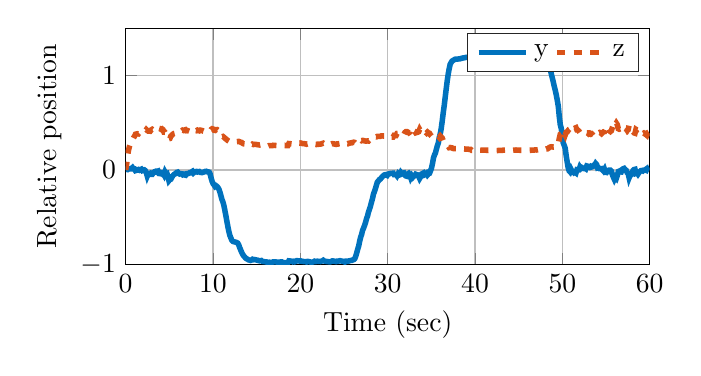
\begin{tikzpicture}

\begin{axis}[%
width=6.656442cm,
height=3cm,
at={(0cm,0cm)},
scale only axis,
xmin=0,
xmax=60,
xlabel={Time (sec)},
xmajorgrids,
ymin=-1,
ymax=1.5,
ylabel={Relative position},
ymajorgrids,
legend style={legend columns=2,legend cell align=left,align=left,draw=white!15!black}
]
\addplot [color=mycolor1,solid,line width=2.0pt]
  table[row sep=crcr]{%
0	0\\
0.112570356472795	0.00731805407497991\\
0.225140712945591	0.00436945945858823\\
0.337711069418386	0.0119259771848855\\
0.450281425891182	0.0109889077497284\\
0.562851782363977	0.0106100106933301\\
0.675422138836773	0.0158729668727864\\
0.787992495309569	0.0253181182206277\\
0.900562851782364	0.0112078244718606\\
1.01313320825516	0.0113160631715622\\
1.12570356472796	-0.00713698458412967\\
1.23827392120075	-0.00381341656223194\\
1.35084427767355	-0.00134275778960943\\
1.46341463414634	0.00421590022255286\\
1.57598499061914	-0.00205884251347951\\
1.68855534709193	0.00448540997813007\\
1.80112570356473	0.00870492599094652\\
1.91369606003752	-0.00633783564470675\\
2.02626641651032	-0.0017439425088126\\
2.13883677298311	0.00100781118503213\\
2.25140712945591	-0.0069112074767913\\
2.36397748592871	-0.0287789657538817\\
2.4765478424015	-0.0648117128803693\\
2.5891181988743	-0.0406773232135265\\
2.70168855534709	-0.0395193318939124\\
2.81425891181989	-0.0346648581541925\\
2.92682926829268	-0.0474066628477943\\
3.03939962476548	-0.0470387884270993\\
3.15196998123827	-0.031758713408384\\
3.26454033771107	-0.0221261393197989\\
3.37711069418386	-0.0231981032784662\\
3.48968105065666	-0.0135190447620132\\
3.60225140712946	-0.0147119650640057\\
3.71482176360225	-0.0112811868877379\\
3.82739212007505	-0.037494040911603\\
3.93996247654784	-0.0390962293403098\\
4.05253283302064	-0.0320582940733466\\
4.16510318949343	-0.0402552942747746\\
4.27767354596623	-0.0319620483377769\\
4.39024390243902	-0.0505848826161995\\
4.50281425891182	-0.0201037087267946\\
4.61538461538462	-0.0384489523082695\\
4.72795497185741	-0.0358538968613467\\
4.84052532833021	-0.0734711979694207\\
4.953095684803	-0.113272365062824\\
5.0656660412758	-0.100870254966162\\
5.17823639774859	-0.0975004479177376\\
5.29080675422139	-0.0783948941846022\\
5.40337711069418	-0.0606268564646574\\
5.51594746716698	-0.0506407265514001\\
5.62851782363977	-0.0418515113102431\\
5.74108818011257	-0.0389145864545959\\
5.85365853658537	-0.0255654345784073\\
5.96622889305816	-0.0227388181164068\\
6.07879924953096	-0.0351322550934524\\
6.19136960600375	-0.0427557807058552\\
6.30393996247655	-0.0392558066661968\\
6.41651031894934	-0.0406392032456923\\
6.52908067542214	-0.0503967523112728\\
6.64165103189493	-0.0454065928917591\\
6.75422138836773	-0.0529951733774885\\
6.86679174484053	-0.0556186829130959\\
6.97936210131332	-0.0401634782611234\\
7.09193245778612	-0.0399925471836716\\
7.20450281425891	-0.0363721782492756\\
7.31707317073171	-0.0295485335463744\\
7.4296435272045	-0.029702615224926\\
7.5422138836773	-0.0214431996454346\\
7.65478424015009	-0.0148413643444097\\
7.76735459662289	-0.0314607884567145\\
7.87992495309569	-0.0226143075842577\\
7.99249530956848	-0.0177319476503696\\
8.10506566604128	-0.0157119828974049\\
8.21763602251407	-0.0215021911022745\\
8.33020637898687	-0.0182245096424719\\
8.44277673545966	-0.016554287158572\\
8.55534709193246	-0.0253409918515133\\
8.66791744840525	-0.0269903220924021\\
8.78048780487805	-0.0271979019496719\\
8.89305816135084	-0.0237010522480463\\
9.00562851782364	-0.0204848826294565\\
9.11819887429644	-0.0153114305972136\\
9.23076923076923	-0.0142324747198221\\
9.34333958724203	-0.019311094070345\\
9.45590994371482	-0.0198332815060534\\
9.56848030018762	-0.0233863564579882\\
9.68105065666041	-0.0455468633313124\\
9.79362101313321	-0.0877741658669943\\
9.906191369606	-0.122481762217677\\
10.0187617260788	-0.146108625321436\\
10.1313320825516	-0.15955177751231\\
10.2439024390244	-0.175021845858156\\
10.3564727954972	-0.167150693475539\\
10.46904315197	-0.175061700497297\\
10.5816135084428	-0.188509553155561\\
10.6941838649156	-0.20631942327936\\
10.8067542213884	-0.237870846841713\\
10.9193245778612	-0.276222557984606\\
11.031894934334	-0.314449086469333\\
11.1444652908068	-0.340493126310703\\
11.2570356472795	-0.379409903431037\\
11.3696060037523	-0.433024507659644\\
11.4821763602251	-0.48654219434092\\
11.5947467166979	-0.545998914247756\\
11.7073170731707	-0.60059773483008\\
11.8198874296435	-0.652055739639487\\
11.9324577861163	-0.692466085324434\\
12.0450281425891	-0.719031394859297\\
12.1575984990619	-0.743941631215646\\
12.2701688555347	-0.755212108128137\\
12.3827392120075	-0.759289233117947\\
12.4953095684803	-0.76193262010704\\
12.6078799249531	-0.764766954463395\\
12.7204502814259	-0.768549916766658\\
12.8330206378987	-0.774553984492752\\
12.9455909943715	-0.792421540348717\\
13.0581613508443	-0.82183362589281\\
13.1707317073171	-0.846780597846666\\
13.2833020637899	-0.871626194411433\\
13.3958724202627	-0.892240495833431\\
13.5084427767355	-0.908738488572267\\
13.6210131332083	-0.919579395909645\\
13.7335834896811	-0.93297500524419\\
13.8461538461538	-0.939180130653608\\
13.9587242026266	-0.945067224490357\\
14.0712945590994	-0.951718356355668\\
14.1838649155722	-0.954654426968431\\
14.296435272045	-0.957358194989526\\
14.4090056285178	-0.952644712623639\\
14.5215759849906	-0.945219009067121\\
14.6341463414634	-0.949799083336535\\
14.7467166979362	-0.948061980898397\\
14.859287054409	-0.950424550833877\\
14.9718574108818	-0.952976711938347\\
15.0844277673546	-0.954301524807797\\
15.1969981238274	-0.958094989756767\\
15.3095684803002	-0.960981602532218\\
15.422138836773	-0.959128946373137\\
15.5347091932458	-0.958279996971421\\
15.6472795497186	-0.9674297909283\\
15.7598499061914	-0.969524907582926\\
15.8724202626642	-0.970542383788034\\
15.984990619137	-0.972060842490218\\
16.0975609756098	-0.971926490690651\\
16.2101313320826	-0.979591880609388\\
16.3227016885553	-0.980656319064104\\
16.4352720450281	-0.976413189963082\\
16.5478424015009	-0.97701861815557\\
16.6604127579737	-0.97874283832266\\
16.7729831144465	-0.97790990723883\\
16.8855534709193	-0.972301283719837\\
16.9981238273921	-0.972297490037528\\
17.1106941838649	-0.972931590002227\\
17.2232645403377	-0.973838094814331\\
17.3358348968105	-0.975390203678056\\
17.4484052532833	-0.976109143053868\\
17.5609756097561	-0.976641765585528\\
17.6735459662289	-0.976580173605269\\
17.7861163227017	-0.972242058858798\\
17.8986866791745	-0.973127161985026\\
18.0112570356473	-0.98001657913437\\
18.1238273921201	-0.980666436308928\\
18.2363977485929	-0.981208888035685\\
18.3489681050657	-0.983837996811948\\
18.4615384615385	-0.983837333901021\\
18.5741088180113	-0.983792104962326\\
18.6866791744841	-0.961736148348128\\
18.7992495309568	-0.962660758219611\\
18.9118198874296	-0.964402905753025\\
19.0243902439024	-0.965882261259264\\
19.1369606003752	-0.971580311900633\\
19.249530956848	-0.966890255745404\\
19.3621013133208	-0.971683223533302\\
19.4746716697936	-0.967193342138042\\
19.5872420262664	-0.959903563574802\\
19.6998123827392	-0.96051929232095\\
19.812382739212	-0.962703798524755\\
19.9249530956848	-0.964221022676541\\
20.0375234521576	-0.961916189095896\\
20.1500938086304	-0.964964142286941\\
20.2626641651032	-0.968513033319437\\
20.375234521576	-0.968853194242371\\
20.4878048780488	-0.970440759145192\\
20.6003752345216	-0.97078596145954\\
20.7129455909944	-0.974643113210212\\
20.8255159474672	-0.968532146349072\\
20.93808630394	-0.968987583752259\\
21.0506566604128	-0.971251417138848\\
21.1632270168856	-0.975372061402467\\
21.2757973733583	-0.975460138896931\\
21.3883677298311	-0.975907326510685\\
21.5009380863039	-0.971826804761919\\
21.6135084427767	-0.96597523469894\\
21.7260787992495	-0.969560994733468\\
21.8386491557223	-0.968783391969902\\
21.9512195121951	-0.965471889927462\\
22.0637898686679	-0.968483472185549\\
22.1763602251407	-0.967856349925358\\
22.2889305816135	-0.968788135483242\\
22.4015009380863	-0.965123614830905\\
22.5140712945591	-0.962592560491468\\
22.6266416510319	-0.955864574318917\\
22.7392120075047	-0.963683035782569\\
22.8517823639775	-0.966279389597772\\
22.9643527204503	-0.966526308272119\\
23.0769230769231	-0.969897253257918\\
23.1894934333959	-0.970851218313718\\
23.3020637898687	-0.971962673224288\\
23.4146341463415	-0.972994064551475\\
23.5272045028143	-0.968495968369534\\
23.6397748592871	-0.963392081776844\\
23.7523452157598	-0.963373399630578\\
23.8649155722326	-0.964769540454916\\
23.9774859287054	-0.96804017282583\\
24.0900562851782	-0.970150915111838\\
24.202626641651	-0.965191821643175\\
24.3151969981238	-0.966045266763434\\
24.4277673545966	-0.962775133863126\\
24.5403377110694	-0.960545305989682\\
24.6529080675422	-0.963218390005046\\
24.765478424015	-0.964747591036602\\
24.8780487804878	-0.966537962220414\\
24.9906191369606	-0.967387390187597\\
25.1031894934334	-0.974856327253224\\
25.2157598499062	-0.965288944406077\\
25.328330206379	-0.966444253880054\\
25.4409005628518	-0.967720571722813\\
25.5534709193246	-0.962579660576044\\
25.6660412757974	-0.960851730360792\\
25.7786116322702	-0.958053519573498\\
25.891181988743	-0.957184800704957\\
26.0037523452158	-0.951606774435013\\
26.1163227016886	-0.948637753206933\\
26.2288930581614	-0.939120716223982\\
26.3414634146341	-0.913098269789105\\
26.4540337711069	-0.877994283753111\\
26.5666041275797	-0.839000713825737\\
26.6791744840525	-0.804674918965404\\
26.7917448405253	-0.754107455446385\\
26.9043151969981	-0.712285683074438\\
27.0168855534709	-0.681621805431276\\
27.1294559099437	-0.637946698676657\\
27.2420262664165	-0.615292562040585\\
27.3545966228893	-0.585910150781077\\
27.4671669793621	-0.554362804732412\\
27.5797373358349	-0.516028376433154\\
27.6923076923077	-0.487043108702936\\
27.8048780487805	-0.444798316810232\\
27.9174484052533	-0.414363019506626\\
28.0300187617261	-0.382441980381661\\
28.1425891181989	-0.341817857375737\\
28.2551594746717	-0.304506348088692\\
28.3677298311445	-0.257151493018888\\
28.4803001876173	-0.228853975229199\\
28.5928705440901	-0.198210227283118\\
28.7054409005629	-0.162527927921652\\
28.8180112570356	-0.1281732804325\\
28.9305816135084	-0.116870526868905\\
29.0431519699812	-0.102674059603913\\
29.155722326454	-0.097495989222061\\
29.2682926829268	-0.0838355763553935\\
29.3808630393996	-0.0719368227023553\\
29.4934333958724	-0.0626165223616686\\
29.6060037523452	-0.0525866757231193\\
29.718574108818	-0.0503654409357598\\
29.8311444652908	-0.0531460533098799\\
29.9437148217636	-0.0582474864400062\\
30.0562851782364	-0.0427502278046333\\
30.1688555347092	-0.0416984139484973\\
30.281425891182	-0.038326863790916\\
30.3939962476548	-0.0351930966469022\\
30.5065666041276	-0.035258840363346\\
30.6191369606004	-0.0339786582892509\\
30.7317073170732	-0.0492809324952892\\
30.844277673546	-0.048255641291341\\
30.9568480300188	-0.0476592380466381\\
31.0694183864916	-0.0615029520718174\\
31.1819887429644	-0.0421211203735031\\
31.2945590994372	-0.0547359307026018\\
31.4071294559099	-0.0505706292913308\\
31.5196998123827	-0.026933726380406\\
31.6322701688555	-0.0389619401195121\\
31.7448405253283	-0.0338450557669276\\
31.8574108818011	-0.0313891980707749\\
31.9699812382739	-0.05440181017766\\
32.0825515947467	-0.0636788185121764\\
32.1951219512195	-0.0664867417288438\\
32.3076923076923	-0.0429733924502976\\
32.4202626641651	-0.0354656035778505\\
32.5328330206379	-0.0473218896279182\\
32.6454033771107	-0.0806394751405874\\
32.7579737335835	-0.0617910304618097\\
32.8705440900563	-0.0771660543649672\\
32.9831144465291	-0.0657423068368676\\
33.0956848030019	-0.0607530742209816\\
33.2082551594747	-0.0452691043009005\\
33.3208255159475	-0.0489158635408173\\
33.4333958724203	-0.0519502587002157\\
33.5459662288931	-0.0670156414935609\\
33.6585365853659	-0.0898601193336011\\
33.7711069418387	-0.0725104775805225\\
33.8836772983114	-0.0428651024548135\\
33.9962476547842	-0.037338469123649\\
34.108818011257	-0.0316200093409963\\
34.2213883677298	-0.0497120524115781\\
34.3339587242026	-0.0429698029678252\\
34.4465290806754	-0.0344823527559307\\
34.5590994371482	-0.0520815946022361\\
34.671669793621	-0.040201324080018\\
34.7842401500938	-0.035950526727173\\
34.8968105065666	-0.00999128090523177\\
35.0093808630394	0.0181498813321691\\
35.1219512195122	0.0636104514180651\\
35.234521575985	0.124033495980031\\
35.3470919324578	0.15714864244027\\
35.4596622889306	0.178420297861652\\
35.5722326454034	0.218152025801048\\
35.6848030018762	0.256412735423268\\
35.797373358349	0.286890255952016\\
35.9099437148218	0.345435965927946\\
36.0225140712946	0.383992705915021\\
36.1350844277674	0.443724888609967\\
36.2476547842402	0.521435334375477\\
36.3602251407129	0.606177793577637\\
36.4727954971857	0.68268134937218\\
36.5853658536585	0.770691608451614\\
36.6979362101313	0.857175538249525\\
36.8105065666041	0.940429603843999\\
36.9230769230769	1.01079646040157\\
37.0356472795497	1.06996921672212\\
37.1482176360225	1.11726717202672\\
37.2607879924953	1.13682109219565\\
37.3733583489681	1.15259937015522\\
37.4859287054409	1.15975760371343\\
37.5984990619137	1.16532170012424\\
37.7110694183865	1.17159469679635\\
37.8236397748593	1.17196089168028\\
37.9362101313321	1.17320447568807\\
38.0487804878049	1.17413836482123\\
38.1613508442777	1.17535326608512\\
38.2739212007505	1.17653660381618\\
38.3864915572233	1.18017703024006\\
38.4990619136961	1.18219171018449\\
38.6116322701689	1.18527593471233\\
38.7242026266417	1.18702668034446\\
38.8367729831145	1.1880883783738\\
38.9493433395872	1.19131654819963\\
39.06191369606	1.19209171504701\\
39.1744840525328	1.19384645122875\\
39.2870544090056	1.19448473129969\\
39.3996247654784	1.19682657228211\\
39.5121951219512	1.19837060066324\\
39.624765478424	1.20917428549723\\
39.7373358348968	1.20941170271446\\
39.8499061913696	1.21150472655647\\
39.9624765478424	1.21184611513885\\
40.0750469043152	1.21471366529071\\
40.187617260788	1.21518338103547\\
40.3001876172608	1.2151737321008\\
40.4127579737336	1.21628926125065\\
40.5253283302064	1.2180006058219\\
40.6378986866792	1.22167332396308\\
40.750469043152	1.22182878804617\\
40.8630393996248	1.22226695670701\\
40.9756097560976	1.22229431813537\\
41.0881801125704	1.22304074590066\\
41.2007504690432	1.22326813715215\\
41.3133208255159	1.22651761177609\\
41.4258911819887	1.22672223377923\\
41.5384615384615	1.22636862426506\\
41.6510318949343	1.22576365912871\\
41.7636022514071	1.22491194236994\\
41.8761726078799	1.22693087343332\\
41.9887429643527	1.22660272641327\\
42.1013133208255	1.22599669477424\\
42.2138836772983	1.22504795460219\\
42.3264540337711	1.22552915721213\\
42.4390243902439	1.2256418861694\\
42.5515947467167	1.22487591927402\\
42.6641651031895	1.22424794506302\\
42.7767354596623	1.22458267446938\\
42.8893058161351	1.22545108397951\\
43.0018761726079	1.22586834719587\\
43.1144465290807	1.22618334177526\\
43.2270168855535	1.22517025754833\\
43.3395872420263	1.22466624260653\\
43.4521575984991	1.22488865157302\\
43.5647279549719	1.22795403401761\\
43.6772983114447	1.22633379578831\\
43.7898686679174	1.2262836165938\\
43.9024390243902	1.22582235759963\\
44.015009380863	1.22566208013689\\
44.1275797373358	1.22509821047593\\
44.2401500938086	1.22767014128426\\
44.3527204502814	1.22620893691877\\
44.4652908067542	1.22389956831749\\
44.577861163227	1.22265020696884\\
44.6904315196998	1.22021503826756\\
44.8030018761726	1.21876751109424\\
44.9155722326454	1.21647983568426\\
45.0281425891182	1.21538949697061\\
45.140712945591	1.21523593569016\\
45.2532833020638	1.21412199225708\\
45.3658536585366	1.21334879421656\\
45.4784240150094	1.21302202642007\\
45.5909943714822	1.2130126004074\\
45.703564727955	1.213206952321\\
45.8161350844278	1.2123024842682\\
45.9287054409006	1.21379578425829\\
46.0412757973734	1.21540566886817\\
46.1538461538462	1.2154864174776\\
46.2664165103189	1.21418352698792\\
46.3789868667917	1.21333587022075\\
46.4915572232645	1.21368854669585\\
46.6041275797373	1.21199217299755\\
46.7166979362101	1.21022178782424\\
46.8292682926829	1.20691652819068\\
46.9418386491557	1.20436821735448\\
47.0544090056285	1.20262591003125\\
47.1669793621013	1.20032595715914\\
47.2795497185741	1.19625490095653\\
47.3921200750469	1.19504260707527\\
47.5046904315197	1.19409667187768\\
47.6172607879925	1.19675055211702\\
47.7298311444653	1.19452806616163\\
47.8424015009381	1.19241632626515\\
47.9549718574109	1.18841947320612\\
48.0675422138837	1.18341657324391\\
48.1801125703565	1.17473778493879\\
48.2926829268293	1.15930425971777\\
48.4052532833021	1.13407051859569\\
48.5178236397749	1.09923330311168\\
48.6303939962477	1.05683512527796\\
48.7429643527204	1.0111827593869\\
48.8555347091933	0.96998528004908\\
48.968105065666	0.926864270675248\\
49.0806754221388	0.880148987006508\\
49.1932457786116	0.839038590399606\\
49.3058161350844	0.791384264186962\\
49.4183864915572	0.735130273583541\\
49.53095684803	0.673793569577783\\
49.6435272045028	0.565326233411874\\
49.7560975609756	0.479903684357385\\
49.8686679174484	0.440217437063586\\
49.9812382739212	0.36092378603283\\
50.093808630394	0.288089543181492\\
50.2063789868668	0.260192443648185\\
50.3189493433396	0.231079194685068\\
50.4315196998124	0.153637983948533\\
50.5440900562852	0.0867242977018263\\
50.656660412758	0.0263986558598818\\
50.7692307692308	-0.00856319785286366\\
50.8818011257036	-0.019960217993458\\
50.9943714821764	0.00409642447611547\\
51.1069418386492	-0.0174616368995152\\
51.219512195122	-0.0169190787650212\\
51.3320825515948	-0.0292894818162276\\
51.4446529080675	-0.0232730197501543\\
51.5572232645403	-0.0314057933916769\\
51.6697936210131	0.00133912730066818\\
51.7823639774859	-0.00116582842808197\\
51.8949343339587	0.000587823761633716\\
52.0075046904315	0.0305585127964207\\
52.1200750469043	0.0156819604589703\\
52.2326454033771	0.0253924046911257\\
52.3452157598499	0.0192250814176059\\
52.4577861163227	0.0154077661179857\\
52.5703564727955	0.0211386085491135\\
52.6829268292683	0.0135711948967951\\
52.7954971857411	0.0423567938828789\\
52.9080675422139	0.039425698965372\\
53.0206378986867	0.0371467918080726\\
53.1332082551595	0.029971830617515\\
53.2457786116323	0.038513698868517\\
53.3583489681051	0.0325996822243984\\
53.4709193245779	0.0371618417556969\\
53.5834896810507	0.0493909191399546\\
53.6960600375235	0.0494719522132658\\
53.8086303939962	0.0685681536688257\\
53.921200750469	0.0569010074133893\\
54.0337711069418	0.0207916829085869\\
54.1463414634146	0.0233159592969207\\
54.2589118198874	0.0146447606231429\\
54.3714821763602	0.0136693615996094\\
54.484052532833	0.0145047298673051\\
54.5966228893058	-6.67272100442762e-05\\
54.7091932457786	-0.0112697608352076\\
54.8217636022514	0.00627720648074168\\
54.9343339587242	-0.0238575750493397\\
55.046904315197	-0.026172502747384\\
55.1594746716698	-0.00820681260360295\\
55.2720450281426	-0.0120089687137519\\
55.3846153846154	-0.00129198598037117\\
55.4971857410882	-0.00179367775729153\\
55.609756097561	-0.0129355399264363\\
55.7223264540338	-0.0489272353098109\\
55.8348968105066	-0.076824834433312\\
55.9474671669794	-0.0992693135413807\\
56.0600375234522	-0.0785435605234452\\
56.172607879925	-0.0895166460479208\\
56.2851782363977	-0.0599432043054638\\
56.3977485928705	-0.0169218908963677\\
56.5103189493433	-0.0121112896350508\\
56.6228893058161	-0.0196851892427727\\
56.7354596622889	-0.0209773278758023\\
56.8480300187617	0.00552728825240487\\
56.9606003752345	0.0128422060729138\\
57.0731707317073	0.0168023523987472\\
57.1857410881801	0.00570228300579698\\
57.2983114446529	-0.00353227698958644\\
57.4108818011257	-0.0281132005574535\\
57.5234521575985	-0.0351601193995077\\
57.6360225140713	-0.0818075562074117\\
57.7485928705441	-0.0552786854865251\\
57.8611632270169	-0.0522316529571216\\
57.9737335834897	-0.0413196060647652\\
58.0863039399625	-0.00526447714509951\\
58.1988742964353	0.00417371069595704\\
58.3114446529081	0.00669817221974289\\
58.4240150093809	-0.0343100215933122\\
58.5365853658537	-0.0298025127830855\\
58.6491557223265	-0.0441390758296234\\
58.7617260787992	-0.0288256765919425\\
58.874296435272	-0.0159415549450407\\
58.9868667917448	-0.00748713191976122\\
59.0994371482176	-0.00587192357088503\\
59.2120075046904	-0.0103264541896632\\
59.3245778611632	-0.00168846731812253\\
59.437148217636	-0.000108224276680474\\
59.5497185741088	0.00587889526294119\\
59.6622889305816	0.0135952388763699\\
59.7748592870544	-0.0114440551810545\\
59.8874296435272	-0.0163201358864677\\
};
\addlegendentry{y};

\addplot [color=mycolor2,dashed,line width=2.0pt]
  table[row sep=crcr]{%
0	0\\
0.112570356472795	0.0603077060262416\\
0.225140712945591	0.151867889531437\\
0.337711069418386	0.21301417677585\\
0.450281425891182	0.254771180132793\\
0.562851782363977	0.284264368614396\\
0.675422138836773	0.303946696900141\\
0.787992495309569	0.321441382252471\\
0.900562851782364	0.341320380344633\\
1.01313320825516	0.355848798753794\\
1.12570356472796	0.378123062328439\\
1.23827392120075	0.38081349400898\\
1.35084427767355	0.382858326296933\\
1.46341463414634	0.381453837563386\\
1.57598499061914	0.392760687445419\\
1.68855534709193	0.392379147048111\\
1.80112570356473	0.393709775330361\\
1.91369606003752	0.407531477801873\\
2.02626641651032	0.40624186018627\\
2.13883677298311	0.406310726230391\\
2.25140712945591	0.412544559104742\\
2.36397748592871	0.427218885712657\\
2.4765478424015	0.416684403825587\\
2.5891181988743	0.410759156750101\\
2.70168855534709	0.411478863468081\\
2.81425891181989	0.409872691148894\\
2.92682926829268	0.42372038357488\\
3.03939962476548	0.429828636893868\\
3.15196998123827	0.421988059450347\\
3.26454033771107	0.419290285790569\\
3.37711069418386	0.418745252962529\\
3.48968105065666	0.41846804161127\\
3.60225140712946	0.423407867887234\\
3.71482176360225	0.419488951751187\\
3.82739212007505	0.440433729189633\\
3.93996247654784	0.437448196737216\\
4.05253283302064	0.430129088771319\\
4.16510318949343	0.434879970640941\\
4.27767354596623	0.426672456415242\\
4.39024390243902	0.399632232639\\
4.50281425891182	0.398740382880377\\
4.61538461538462	0.379107232204309\\
4.72795497185741	0.379222454936733\\
4.84052532833021	0.372459146368266\\
4.953095684803	0.329320393402299\\
5.0656660412758	0.332731088029694\\
5.17823639774859	0.358563225835145\\
5.29080675422139	0.3669236046506\\
5.40337711069418	0.378565358860316\\
5.51594746716698	0.385444777802976\\
5.62851782363977	0.387844802077567\\
5.74108818011257	0.38793769556063\\
5.85365853658537	0.394819338090212\\
5.96622889305816	0.392763485027147\\
6.07879924953096	0.3996309994176\\
6.19136960600375	0.406935575769703\\
6.30393996247655	0.406278224495607\\
6.41651031894934	0.411126964945436\\
6.52908067542214	0.420744924849644\\
6.64165103189493	0.41719061713407\\
6.75422138836773	0.423267883995486\\
6.86679174484053	0.426613728001495\\
6.97936210131332	0.415543413151947\\
7.09193245778612	0.416489724852055\\
7.20450281425891	0.412906655130341\\
7.31707317073171	0.408893408108959\\
7.4296435272045	0.419057403814182\\
7.5422138836773	0.417516298148458\\
7.65478424015009	0.413583399082203\\
7.76735459662289	0.429870526246137\\
7.87992495309569	0.421834663680533\\
7.99249530956848	0.417464882244129\\
8.10506566604128	0.415673217460649\\
8.21763602251407	0.421882546808393\\
8.33020637898687	0.417473473325124\\
8.44277673545966	0.414209555881893\\
8.55534709193246	0.421575208888981\\
8.66791744840525	0.419581259987672\\
8.78048780487805	0.416423407150787\\
8.89305816135084	0.410826059621549\\
9.00562851782364	0.408424007040834\\
9.11819887429644	0.409428872995965\\
9.23076923076923	0.408030141580983\\
9.34333958724203	0.411222929632328\\
9.45590994371482	0.410664874726136\\
9.56848030018762	0.411695782722678\\
9.68105065666041	0.412596585246162\\
9.79362101313321	0.429005689223382\\
9.906191369606	0.435977379826057\\
10.0187617260788	0.432538402900535\\
10.1313320825516	0.420149768378415\\
10.2439024390244	0.418352411938455\\
10.3564727954972	0.426935069133992\\
10.46904315197	0.427613788941584\\
10.5816135084428	0.419596739453685\\
10.6941838649156	0.408116085205398\\
10.8067542213884	0.38846768937909\\
10.9193245778612	0.363169858779851\\
11.031894934334	0.350325987116653\\
11.1444652908068	0.354180309925972\\
11.2570356472795	0.346035986943069\\
11.3696060037523	0.335228813892605\\
11.4821763602251	0.328521239445995\\
11.5947467166979	0.31907696495502\\
11.7073170731707	0.310814711554326\\
11.8198874296435	0.304705475814599\\
11.9324577861163	0.300102898738257\\
12.0450281425891	0.302619042859885\\
12.1575984990619	0.297479121440398\\
12.2701688555347	0.296784343710756\\
12.3827392120075	0.297251296680666\\
12.4953095684803	0.29866582066191\\
12.6078799249531	0.298882592874749\\
12.7204502814259	0.299711280089999\\
12.8330206378987	0.300622562795977\\
12.9455909943715	0.302506048565927\\
13.0581613508443	0.297923790826131\\
13.1707317073171	0.294309925900671\\
13.2833020637899	0.291261295038807\\
13.3958724202627	0.281750070831199\\
13.5084427767355	0.276904418063741\\
13.6210131332083	0.275853627708427\\
13.7335834896811	0.269525026523918\\
13.8461538461538	0.267774303717786\\
13.9587242026266	0.264130737723749\\
14.0712945590994	0.260761888652198\\
14.1838649155722	0.259713308419575\\
14.296435272045	0.259423926825685\\
14.4090056285178	0.265304890188578\\
14.5215759849906	0.273365951277572\\
14.6341463414634	0.269380743062609\\
14.7467166979362	0.271577667058956\\
14.859287054409	0.270339835016541\\
14.9718574108818	0.269398230983963\\
15.0844277673546	0.268605152447285\\
15.1969981238274	0.265843231742845\\
15.3095684803002	0.264151108998378\\
15.422138836773	0.266324051529383\\
15.5347091932458	0.268324571476141\\
15.6472795497186	0.264460744399093\\
15.7598499061914	0.263348035161373\\
15.8724202626642	0.262379076674936\\
15.984990619137	0.261646010472828\\
16.0975609756098	0.260585799010057\\
16.2101313320826	0.255350013983156\\
16.3227016885553	0.254237514894278\\
16.4352720450281	0.25857197675773\\
16.5478424015009	0.258646682615412\\
16.6604127579737	0.256977258600847\\
16.7729831144465	0.256624249532383\\
16.8855534709193	0.261165214100454\\
16.9981238273921	0.259976994225431\\
17.1106941838649	0.259449122177281\\
17.2232645403377	0.258713088432857\\
17.3358348968105	0.257895175213048\\
17.4484052532833	0.25808545529933\\
17.5609756097561	0.258008229393757\\
17.6735459662289	0.258572607873906\\
17.7861163227017	0.263151732868743\\
17.8986866791745	0.263345982482317\\
18.0112570356473	0.259440236477252\\
18.1238273921201	0.258962348365796\\
18.2363977485929	0.259238531736538\\
18.3489681050657	0.257384856452357\\
18.4615384615385	0.257365505808837\\
18.5741088180113	0.257380118447124\\
18.6866791744841	0.279262079853372\\
18.7992495309568	0.278352162846845\\
18.9118198874296	0.276765131728984\\
19.0243902439024	0.275484267668735\\
19.1369606003752	0.275408572904996\\
19.249530956848	0.277451804689929\\
19.3621013133208	0.273667346992814\\
19.4746716697936	0.277974034360159\\
19.5872420262664	0.285325485825941\\
19.6998123827392	0.286453686721646\\
19.812382739212	0.284413330600374\\
19.9249530956848	0.283021009032894\\
20.0375234521576	0.285120000398031\\
20.1500938086304	0.282057748850123\\
20.2626641651032	0.279284010785879\\
20.375234521576	0.278844031668577\\
20.4878048780488	0.277116803559191\\
20.6003752345216	0.276890862329178\\
20.7129455909944	0.272636352742531\\
20.8255159474672	0.27587118260305\\
20.93808630394	0.275597583412783\\
21.0506566604128	0.273963760784397\\
21.1632270168856	0.270630781659148\\
21.2757973733583	0.270574722191552\\
21.3883677298311	0.270120465634925\\
21.5009380863039	0.274262573391923\\
21.6135084427767	0.274691477954826\\
21.7260787992495	0.271123009704914\\
21.8386491557223	0.269314613559166\\
21.9512195121951	0.272874998612288\\
22.0637898686679	0.27085010493343\\
22.1763602251407	0.273418286222593\\
22.2889305816135	0.272815251069814\\
22.4015009380863	0.27672417016575\\
22.5140712945591	0.27967173402632\\
22.6266416510319	0.283345192735935\\
22.7392120075047	0.276753361541237\\
22.8517823639775	0.274221593023981\\
22.9643527204503	0.274009694141926\\
23.0769230769231	0.270834005726158\\
23.1894934333959	0.270369109197655\\
23.3020637898687	0.269330182423155\\
23.4146341463415	0.26800004066617\\
23.5272045028143	0.273152875447419\\
23.6397748592871	0.278156803034656\\
23.7523452157598	0.277313927460033\\
23.8649155722326	0.275801876823848\\
23.9774859287054	0.272759064580537\\
24.0900562851782	0.270772502132005\\
24.202626641651	0.275609472679025\\
24.3151969981238	0.274750374991014\\
24.4277673545966	0.278072873692324\\
24.5403377110694	0.280024701379732\\
24.6529080675422	0.277692656764787\\
24.765478424015	0.276117672958424\\
24.8780487804878	0.274322303123132\\
24.9906191369606	0.273625927659128\\
25.1031894934334	0.269712648834547\\
25.2157598499062	0.2791431571827\\
25.328330206379	0.27806622096793\\
25.4409005628518	0.277219589613482\\
25.5534709193246	0.282425314811496\\
25.6660412757974	0.284301396099637\\
25.7786116322702	0.286837415109412\\
25.891181988743	0.286982788464833\\
26.0037523452158	0.292329416472767\\
26.1163227016886	0.293774097086368\\
26.2288930581614	0.291166390158774\\
26.3414634146341	0.281841068929217\\
26.4540337711069	0.287434234896881\\
26.5666041275797	0.287803321663551\\
26.6791744840525	0.28601052108603\\
26.7917448405253	0.300746893937773\\
26.9043151969981	0.317221637137639\\
27.0168855534709	0.309657895151825\\
27.1294559099437	0.313040990589881\\
27.2420262664165	0.311125831718046\\
27.3545966228893	0.307675588831236\\
27.4671669793621	0.305812582929042\\
27.5797373358349	0.305139619517031\\
27.6923076923077	0.307674361292765\\
27.8048780487805	0.306298031379519\\
27.9174484052533	0.31800428268895\\
28.0300187617261	0.321710923978449\\
28.1425891181989	0.328008487093504\\
28.2551594746717	0.330268121113967\\
28.3677298311445	0.338239095951149\\
28.4803001876173	0.352871106628732\\
28.5928705440901	0.351233432271677\\
28.7054409005629	0.350119626165565\\
28.8180112570356	0.355665267740642\\
28.9305816135084	0.355358367034475\\
29.0431519699812	0.356182059599064\\
29.155722326454	0.35601828963596\\
29.2682926829268	0.360568016073351\\
29.3808630393996	0.361032302236733\\
29.4934333958724	0.359423009395986\\
29.6060037523452	0.359283789744964\\
29.718574108818	0.358939592421665\\
29.8311444652908	0.356744336853429\\
29.9437148217636	0.363699552810265\\
30.0562851782364	0.353866987942544\\
30.1688555347092	0.350372389392055\\
30.281425891182	0.352435911760249\\
30.3939962476548	0.349041552800632\\
30.5065666041276	0.348782249335507\\
30.6191369606004	0.348188907001582\\
30.7317073170732	0.366288067494543\\
30.844277673546	0.365148945738593\\
30.9568480300188	0.364283262759793\\
31.0694183864916	0.386115172278806\\
31.1819887429644	0.386886228257366\\
31.2945590994372	0.397540796399012\\
31.4071294559099	0.393172544843607\\
31.5196998123827	0.377751324361665\\
31.6322701688555	0.382052165014413\\
31.7448405253283	0.37798450381652\\
31.8574108818011	0.375073102341657\\
31.9699812382739	0.397287072010633\\
32.0825515947467	0.405442307399633\\
32.1951219512195	0.405719234636149\\
32.3076923076923	0.401352111372221\\
32.4202626641651	0.393197577976972\\
32.5328330206379	0.40060081333766\\
32.6454033771107	0.43389519628611\\
32.7579737335835	0.414268069546841\\
32.8705440900563	0.426113494725582\\
32.9831144465291	0.413391306133417\\
33.0956848030019	0.408354986025551\\
33.2082551594747	0.392982230503739\\
33.3208255159475	0.396471852685421\\
33.4333958724203	0.39867861689904\\
33.5459662288931	0.403955147120674\\
33.6585365853659	0.42908679165114\\
33.7711069418387	0.410851733115429\\
33.8836772983114	0.402462065218472\\
33.9962476547842	0.396498876522625\\
34.108818011257	0.391554481885181\\
34.2213883677298	0.407454320735675\\
34.3339587242026	0.399557666180258\\
34.4465290806754	0.390116320201386\\
34.5590994371482	0.401400269126122\\
34.671669793621	0.393109200602789\\
34.7842401500938	0.389302955077704\\
34.8968105065666	0.369915301472475\\
35.0093808630394	0.360866608914416\\
35.1219512195122	0.346131177773626\\
35.234521575985	0.340871312352927\\
35.3470919324578	0.343794630416821\\
35.4596622889306	0.35005444238417\\
35.5722326454034	0.351315380672321\\
35.6848030018762	0.348691946029668\\
35.797373358349	0.355950797927098\\
35.9099437148218	0.343708944885639\\
36.0225140712946	0.359145544138419\\
36.1350844277674	0.347786035652971\\
36.2476547842402	0.33663160764953\\
36.3602251407129	0.309874648488172\\
36.4727954971857	0.299563527626196\\
36.5853658536585	0.289388140158279\\
36.6979362101313	0.269464711754513\\
36.8105065666041	0.259703016175031\\
36.9230769230769	0.250239654265727\\
37.0356472795497	0.235595686746125\\
37.1482176360225	0.237576583280366\\
37.2607879924953	0.235190735140304\\
37.3733583489681	0.233458224499819\\
37.4859287054409	0.227292906995644\\
37.5984990619137	0.22492010248195\\
37.7110694183865	0.225530197048919\\
37.8236397748593	0.225602025717922\\
37.9362101313321	0.226619067139522\\
38.0487804878049	0.226755852438094\\
38.1613508442777	0.227099551598636\\
38.2739212007505	0.226987366136966\\
38.3864915572233	0.223801489885681\\
38.4990619136961	0.223318558052055\\
38.6116322701689	0.222010628822415\\
38.7242026266417	0.222283596462672\\
38.8367729831145	0.22176591968626\\
38.9493433395872	0.219818817557584\\
39.06191369606	0.219615997053773\\
39.1744840525328	0.219522544230711\\
39.2870544090056	0.218911378951737\\
39.3996247654784	0.216611790265302\\
39.5121951219512	0.216699215423197\\
39.624765478424	0.20780039298201\\
39.7373358348968	0.207899105253181\\
39.8499061913696	0.207591357255667\\
39.9624765478424	0.207818497121792\\
40.0750469043152	0.212715664279218\\
40.187617260788	0.213421389865052\\
40.3001876172608	0.21303445744811\\
40.4127579737336	0.211800376298387\\
40.5253283302064	0.210972978759853\\
40.6378986866792	0.210621324306876\\
40.750469043152	0.209778120868741\\
40.8630393996248	0.209739207505689\\
40.9756097560976	0.209884978417616\\
41.0881801125704	0.210172262599785\\
41.2007504690432	0.210365899817396\\
41.3133208255159	0.208221804631298\\
41.4258911819887	0.208563043680445\\
41.5384615384615	0.208710198467511\\
41.6510318949343	0.209055088847248\\
41.7636022514071	0.208580967591786\\
41.8761726078799	0.208374207287809\\
41.9887429643527	0.207971204995296\\
42.1013133208255	0.207577842441813\\
42.2138836772983	0.208036728831922\\
42.3264540337711	0.205798472773961\\
42.4390243902439	0.204894059738448\\
42.5515947467167	0.204957611803811\\
42.6641651031895	0.206617208668956\\
42.7767354596623	0.206646712635482\\
42.8893058161351	0.207868711570341\\
43.0018761726079	0.207120892828338\\
43.1144465290807	0.207611339461146\\
43.2270168855535	0.209688511675876\\
43.3395872420263	0.209655697022058\\
43.4521575984991	0.210398217945395\\
43.5647279549719	0.207130712442652\\
43.6772983114447	0.207514545326811\\
43.7898686679174	0.207711299602246\\
43.9024390243902	0.211862852497584\\
44.015009380863	0.211933067192778\\
44.1275797373358	0.211858290969158\\
44.2401500938086	0.208900030526535\\
44.3527204502814	0.209726126851868\\
44.4652908067542	0.210774644332914\\
44.577861163227	0.209956915820802\\
44.6904315196998	0.211174559657591\\
44.8030018761726	0.210679454917035\\
44.9155722326454	0.209216674106229\\
45.0281425891182	0.209069892439454\\
45.140712945591	0.208422425833311\\
45.2532833020638	0.208527911314333\\
45.3658536585366	0.208718656900711\\
45.4784240150094	0.20901349591523\\
45.5909943714822	0.20994970877153\\
45.703564727955	0.210195764034209\\
45.8161350844278	0.210936420016647\\
45.9287054409006	0.208764789420004\\
46.0412757973734	0.20790063064609\\
46.1538461538462	0.207729133647925\\
46.2664165103189	0.208402827756523\\
46.3789868667917	0.208515100522923\\
46.4915572232645	0.209103220627717\\
46.6041275797373	0.209485826427517\\
46.7166979362101	0.210769701011529\\
46.8292682926829	0.211289063622958\\
46.9418386491557	0.212358808726735\\
47.0544090056285	0.21129482530328\\
47.1669793621013	0.212302396578469\\
47.2795497185741	0.214286717137971\\
47.3921200750469	0.213675410833369\\
47.5046904315197	0.216106122444775\\
47.6172607879925	0.219646632214286\\
47.7298311444653	0.219181055660738\\
47.8424015009381	0.218005166967943\\
47.9549718574109	0.217791531726519\\
48.0675422138837	0.21918012744981\\
48.1801125703565	0.223582248249025\\
48.2926829268293	0.223298650915597\\
48.4052532833021	0.229556382455265\\
48.5178236397749	0.238907436410169\\
48.6303939962477	0.24338443741681\\
48.7429643527204	0.245327302423809\\
48.8555347091933	0.244321151658211\\
48.968105065666	0.242097600111604\\
49.0806754221388	0.243224620629909\\
49.1932457786116	0.250917952925941\\
49.3058161350844	0.25308415238523\\
49.4183864915572	0.266532925808042\\
49.53095684803	0.27642429965821\\
49.6435272045028	0.332151750834331\\
49.7560975609756	0.377526735543302\\
49.8686679174484	0.383524372428565\\
49.9812382739212	0.410332276165098\\
50.093808630394	0.417577601568974\\
50.2063789868668	0.392030971473673\\
50.3189493433396	0.369460874924782\\
50.4315196998124	0.398736053854531\\
50.5440900562852	0.40199689148376\\
50.656660412758	0.417017229040446\\
50.7692307692308	0.430434804638372\\
50.8818011257036	0.436843943026786\\
50.9943714821764	0.41056135648694\\
51.1069418386492	0.428711527938214\\
51.219512195122	0.425154220469395\\
51.3320825515948	0.437139345005079\\
51.4446529080675	0.442470122892781\\
51.5572232645403	0.447126984942822\\
51.6697936210131	0.422635078758579\\
51.7823639774859	0.420999606688818\\
51.8949343339587	0.411371002320581\\
52.0075046904315	0.395694328939621\\
52.1200750469043	0.399173446336599\\
52.2326454033771	0.388484313072288\\
52.3452157598499	0.39751805797458\\
52.4577861163227	0.4013959102231\\
52.5703564727955	0.392816340567065\\
52.6829268292683	0.396380612373034\\
52.7954971857411	0.392861878051413\\
52.9080675422139	0.393040530973316\\
53.0206378986867	0.381897240883677\\
53.1332082551595	0.388073527490282\\
53.2457786116323	0.379083144006792\\
53.3583489681051	0.383310366143648\\
53.4709193245779	0.373518487137941\\
53.5834896810507	0.362328045266185\\
53.6960600375235	0.360047708307376\\
53.8086303939962	0.360625455618613\\
53.921200750469	0.367912279936552\\
54.0337711069418	0.397335463452064\\
54.1463414634146	0.392193215273377\\
54.2589118198874	0.397214763973997\\
54.3714821763602	0.393173287205802\\
54.484052532833	0.384257598034478\\
54.5966228893058	0.394140981098979\\
54.7091932457786	0.403065308188147\\
54.8217636022514	0.405558703034763\\
54.9343339587242	0.432528185886429\\
55.046904315197	0.462423517129632\\
55.1594746716698	0.429858691051471\\
55.2720450281426	0.429942071653344\\
55.3846153846154	0.413654888349952\\
55.4971857410882	0.406342358622931\\
55.609756097561	0.415207445149181\\
55.7223264540338	0.450813938783089\\
55.8348968105066	0.477420675737206\\
55.9474671669794	0.497700828179925\\
56.0600375234522	0.477367874996512\\
56.172607879925	0.495897780496607\\
56.2851782363977	0.480038920295667\\
56.3977485928705	0.436490197664796\\
56.5103189493433	0.431087636209572\\
56.6228893058161	0.434904622356363\\
56.7354596622889	0.433735812637592\\
56.8480300187617	0.405471974621933\\
56.9606003752345	0.393940096512626\\
57.0731707317073	0.383246709133872\\
57.1857410881801	0.392778148937236\\
57.2983114446529	0.398973679235347\\
57.4108818011257	0.41881278261812\\
57.5234521575985	0.425588894587939\\
57.6360225140713	0.472340458955485\\
57.7485928705441	0.445169888325911\\
57.8611632270169	0.441039952417573\\
57.9737335834897	0.423732427553936\\
58.0863039399625	0.404426091267919\\
58.1988742964353	0.392765826463791\\
58.3114446529081	0.389109791082437\\
58.4240150093809	0.42932312129282\\
58.5365853658537	0.422446668014053\\
58.6491557223265	0.431004001051196\\
58.7617260787992	0.408652942822085\\
58.874296435272	0.395448336529024\\
58.9868667917448	0.385677143290481\\
59.0994371482176	0.381305199644344\\
59.2120075046904	0.384133438027598\\
59.3245778611632	0.39019592442696\\
59.437148217636	0.382280708672057\\
59.5497185741088	0.37554773385429\\
59.6622889305816	0.366784503737469\\
59.7748592870544	0.39455314338644\\
59.8874296435272	0.400127673758939\\
};
\addlegendentry{z};

\end{axis}
\end{tikzpicture}%
      \caption{Relative position between the cross product and the principal lines }
    \label{fig:LateralPosition}
  \end{figure}

  \color{black}
%

\section{Conclusions}
